\documentclass[11pt]{article}
%\usepackage{helvet}
\usepackage{lastpage, fancyhdr,color,amsmath,amssymb,amsfonts,amscd, graphicx,latexsym,multirow}
\usepackage{makecell}
\usepackage{eurosym}
\usepackage[all]{xy}
\pagestyle{empty}
%\usepackage[turkish]{babel}
\usepackage[utf8]{inputenc}
\usepackage[T1]{fontenc}
\setlength\voffset{-1in}
\setlength\hoffset{-1in}
\setlength\topmargin{3cm}
\setlength\oddsidemargin{2.5cm}
\setlength\textheight{8in}
\setlength\textwidth{6.51in}
\setlength\footskip{1in}
\setlength\headheight{12pt}
\setlength\headsep{0.06in}
\usepackage{tikz}
%plus4mm minus3mm}
\usepackage{caption, subcaption, amsfonts}
\usepackage{setspace}
\usepackage{epstopdf}
\usepackage{relsize}
\usepackage{pgf, float}
\usepackage{url}
\newcommand{\gal}{Gal({\mathbb Q})}
\newcommand{\N}{\mathbb N}
\newcommand{\F}{\mathcal F}
\renewcommand{\H}{\mathcal H}
\newcommand{\Q}{\mathbb Q}
\newcommand{\Z}{\mathbb Z}
\newcommand{\R}{\mathbb R} 
\newcommand{\C}{\mathbb C}
\newcommand{\p}{\mathbb P}
\newcommand{\B}{\mathbb B}
\def\modorb{\mbox{$\otimes\hspace{-1.5mm}-\!\!\!-\!\!\!-\hspace{-1.5mm}\circledast$}}
\hyphenation{or-bi-fold}
%\input{defs.tex}

%\usepackage[usenames,dvipsnames]{color}
%\usepackage{epsfig}


% ’

\definecolor{light-gray}{gray}{0.55}
\newcommand\Note[1]{\textcolor{red}{{#1}}}
\begin{document}
\pagestyle{fancy}
   \lhead{}\rhead{}
   \lfoot{\textcolor{light-gray}{\small Proje Sonuç Raporu}}
        \cfoot{{\thepage}}
        \rfoot{}
  \renewcommand{\headrulewidth}{0pt}
%  \renewcommand{\footrulewidth}{0.4pt}
%\def\HG{{\bf HG-GalAct }}

\label{coverpage}

\renewcommand{\figurename}{\bf Şekil}
\renewcommand{\tablename}{\bf Tablo}
\renewcommand{\contentsname}{İçindekiler}
\renewcommand{\refname}{Referanslar}
\renewcommand{\listfigurename}{Şekiller}
\renewcommand{\listtablename}{Tablolar}
%\renewcommand{\familydefault}{\sfdefault}

\newpage
\phantom{22}
\vspace{-3cm}

% % % {\selectlanguage{turkish}\bfseries\color{red} \small Başvuru Formunun ``Bütçe ve Gerekçesi (13. Madde)'' dışındaki bölümleri toplamda Arial, 9 yazı tipinde 20 sayfayı geçmemelidir!}
% % % 
% % % \begin{center}
% % % 	\selectlanguage{turkish}\bfseries \footnotesize Kariyer proje önerisi değerlendirme formuna \\ \url{http://www.tubitak.gov.tr/tubitak_content_files/ARDEB/destek_prog/danisman_panelist/3501_DA_Panelist_Proje_Onerisi_Degerlendirme_Formu.doc} \\
% % % 	adresinden ulaşabilirsiniz.
% % % \end{center}


\begin{center}

\includegraphics[keepaspectratio]{tubitak.png}

\bigskip
\bigskip


\bigskip
{\fontsize{15}{10}\selectfont 
\bigskip


\bigskip
\medskip
{ \textbf{\Huge Birden Fazla Veri Kaynağı Kullanabilen Yeni Genom Birleştirme Algoritmalarının Tasarımı Ve Uygulanması \\}}}


\bigskip
\medskip
{ \textbf{ PROJE SONUÇ RAPORU}}
\bigskip





\end{center}


\bigskip

\bigskip


\thispagestyle{empty}


\begin{center}
\medskip
{\LARGE \textbf{Program Kodu:} 1001}

\bigskip
{\LARGE \textbf{Proje No:} 112E135}

\bigskip
{\LARGE Proje Yürütücüsü:\\
\textbf{Can Alkan}}

\end{center}



\bigskip


\bigskip
\noindent
{\large
\noindent
\underline{\bf Bursiyerler:}

\noindent
Shatlyk Ashyralyyev

\noindent
Fatma Balcı (Kahveci)

\noindent
Elif Dal

\noindent \underline{\bf Projeden desteklenmeyen diğer araştırmacılar:}

\noindent
Pınar Kavak: Destekleyen kurum (TÜBİTAK İGBAM) çalışanı ve Boğaziçi Üniversitesi öğrencisi

\noindent
Can Fırtına: Bilkent Üniversitesi lisans öğrencisi (proje sırasında)


}



\bigskip





\begin{center}
{\Large NİSAN 2016

\vspace{1mm}
ANKARA}
\end{center}


\linespread{1.5}

\newpage\setlength{\parskip}{3mm} 
\onehalfspacing
\bigskip
\pagenumbering{roman}
\setcounter{page}{1}
\begin{center}
{\LARGE \bf ÖNSÖZ}
\end{center}
\addcontentsline{toc}{section}{ÖNSÖZ}


Proje süresince proje ekibinin şu yayınları hazırlanmıştır: 

\begin{itemize}
\item Early post-zygotic mutations contribute to de novo variation in a healthy monozygotic twin pair. G.M. Dal, B. Ergüner, M. S. Sağıroğlu, B. Yüksel, O. E. Onat, {\bf C. Alkan}, T. Özçelik. Journal of Medical Genetics, 51:455-459, 2014.
\item Whole genome sequencing of Turkish genomes reveals functional private alleles and impact of genetic interactions with Europe, Asia and Africa. {\bf C. Alkan}, P.  Kavak, M. Somel, O. Gokcumen, 
  S. Uğurlu, C. Saygı, {\bf E. Dal}, K. Buğra-Bilge,  T. Güngör, S. C. Sahinalp, N. Özören, C. Bekpen. BMC Genomics, 15(1):963, 2014.
\end{itemize}

Proje süresince proje ekibinin şu bildiriler sunulmuştur:
 
\begin{itemize}
\item A hypergraph model for hybrid genome assembly. {\bf S. Ashyralyyev}, C. Firtina, C. Aykanat, {\bf C. Alkan}. Bertinoro Computational Biology Meeting, 14-18 May 2015, Bertinoro, Italy. (özet bildiri)
\item Improving genome assemblies using multi-platform sequence data.
{\bf P. Kavak}, B. Ergüner, D. Üstek, B. Yüksel, M.Ş. Sağıroğlu, T. Güngör, {\bf C. Alkan}.
{\em Proceedings of the $12^{th}$ Computational Intelligence methods for Bioinformatics and Biostatistics (CIBB 2015)}, 
 September 10-12, 2015, Naples, Italy. (tam bildiri)
\end{itemize}

Proje kapsamında desteklenen aşağıdaki bursiyerler,  lisansüstü eğitimlerini 
proje yürütücüsünün danışmanlığında
yapmıştır.
 
\begin{itemize}
\item Fatma Kahveci (Balcı), Bilkent Üniversitesi Bilgisayar Mühendisliği, Yüksek Lisans, Ağustos 2014.
\item Elif Dal, Bilkent Üniversitesi Bilgisayar Mühendisliği, Yüksek Lisans, Aralık 2014.
\end{itemize}


\bigskip
\hfill Can Alkan

\hfill Ankara, Nisan 2016
\newpage

\setlength{\parskip}{1mm} 

\tableofcontents
\listoffigures
\listoftables



\newpage \setlength{\parskip}{3mm}
\phantom{ss}
\vspace{-2.5cm}

\begin{center}
{\bf \Large ÖZET} 
\end{center}
\addcontentsline{toc}{section}{ÖZET}
\noindent

Yeni nesil dizileme (YND) teknolojilerinin uygulanması genomiks alanını kökten değiştirmektedir. Farklı türlerin genomlarını incelemede ve gerek normal gerekse hastalığa yol açan insanlardaki genetik farklılıkların incelenmesinde önceden beklenmeyen derecede çözünürlük sağlamaktadır. Her ne kadar YND verilerinin analizi için çok önemli gelişmeler olmuşsa da, halen YND yöntemlerinin tüm gücünden faydalanılmasının önünde engeller vardır.

Önceden hayal dahi edilemeyecek hızda verileri günümüzde üretebiliyor olmamıza rağmen, bu verilerin analizleri çok daha yavaş hızda olmaktadır. Çünkü 1) emsalsiz miktarlardaki veriler bilişimsel altyapılarda hem verilerin saklanması hem de işlenmesi açısından sorunlar doğurmaktadır; 2) YND platformları tarafından üretilen dizi parçaları genelde yüksek oranda hata içermektedir ve bu parçalar çok kısadır; 3) hem halihazırda kullanılmakta olan algoritmalar hem de YND platformları genomun bazı farklı yapıdaki bölgelerinde düşük performanslı çalışmaktadırlar. İşte bu nedenlerden ötürü dizileme verilerinde var olan bilgiler tamamen kullanılamamaktadır. Bu çok miktardaki verilerin daha iyi işlenmesi ve YND yöntemlerinin gerçek gücünün ortaya çıkarılması için bilgisayar bilimleri ve genomiks arasında bir işbirliğinin kurulması gerekmektedir.

Genom dizileme maliyetinin büyük ölçüde düşmesi sayesinde farklı organizmalar arasındaki genomik çeşitliliğin, organizmal biyolojinin ve genom evriminin daha iyi anlaşılması için binlerce farklı türün genomlarının dizilenmesine yönelik büyük bir ilgi vardır. Son bir kaç yılda bir çok genom, örneğin pirinç, üzüm, buğday, patates, mısır ve salatalık gibi bitkiler; panda, hindi, goril, orangutan, bonobo, keseli sıçan (opossum) ve fil gibi hayvanların genomlari dizilenmistir. Yakın zamanda Genome 10K gibi çok iddialı projeler başlamış ve 10.000 omurgalı hayvanın tüm genom dizilenmesinin yapılması amaçlanmıştır. Ancak YDS platformlarıyla üretilen verilerin yukarıda bahsedilen sınırları farklı türlerin referans genomlarının ortaya çıkarılmasını amaçlayan yeni dizileme çalışmalarını da (de novo sequencing) olumsuz etkilemektedir. Bunun başlıca nedenleri çoğu türün genomlarında aynı ya da benzer DNA dizilerinin genomun farklı yerlerinde tekrarlanması, YND verilerindeki dizi parçacıklarının (sequence read) kısa olması ve yüksek oranda hataların bulunmasıdır. Bu nedenle tüm genom dizilerinin çıkarılması sırasındaki genom birleştirmenin (genome assembly) doğruluğunun arttırılması için halen çözülmesi gereken problemler bulunmaktadır. Dizilenmiş genomların doğruluğu yetersiz derecede olursa, bu genomların incelenmesinden çıkarılacak biyolojik sonuçlar da hatalı olacaktır.

Bu projede birden fazla veri türünü birlikte kullanabilecek algoritmaların tasarlanmasını ve uygulanmasını hedefledik. Farklı şekillerde üretilmiş genom dizileme verilerinin gösterdiği farklı özellikleri aynı anda kullanarak ortaya çıkarılacak referans genomlarının kalitesinin arttırılması için çeşitli yöntemler üzerinde çalıştık. Böylece bu proje dahilinde üretmeye başladığımız gelişmiş algoritmalar yeni dizilenmiş genomları daha iyi birleştirmemizi sağlayacak ve genom biyolojilerini daha iyi anlamamıza yardımcı olacaktır. 

Bu proje dahilinde dört ana amaç üzerinde çalıştık. 
Birincisi, önceden geliştirilmiş olan iskeleleme algoritmalarının birden fazla veri tipi ve havuzlanmış klon dizileme verileri kullanıldığında genom birleştirmelerine faydalı etkisinin incelenmesiydi (Elif Dal, Yüksek Lisans Tezi). İkincisi Illumina, Roche/454 ve Ion Torrent verilerini birlikte kullanarak geliştirdiğimiz bir genom birleştirme hata düzeltme algoritmasıydı ve bu algoritmayı bir bakteri yapak kromozomu üzerinde denedik (Pınar Kavak, doktora projesi -- sürüyor).
Üçüncü projemiz Illumina verileri kullanılarak PacBio verilerindeki hataların düzeltilmesi (Can Fırtına, CS490: Bilgisayar Mühendisliği ve Biliminde Araştırmaya Giriş dersi projesi) ve düzeltilmiş PacBio verileri ile Illumina verilerinin eşzamanlı olarak bir hiperçizge üzerinde ifadesi ile genom birleştirmesi yapılmasıdır (Shatlyk Ashyralyyev, doktora tezi -- sürüyor). Son olarak Illumina platformunda ortaya çıkan GC oranlarının yüksek ve düşük olduğu bölgelerdeki dizileme derinliğindeki sapmaların düzeltilmesi ve özellikle ekzom dizilemedeki hataların giderilmesi, böylece ekzom birleştirmelerinin iyileştirilmesi üzerine çalıştık (Fatma Balcı, Yüksek Lisans Tezi). 

{\bf Anahtar kelimeler:} genomiks, yeni nesil dizileme, genom birleştirme, algoritmalar, çizge kuramı

\newpage
\phantom{ss}
\vspace{-2.5cm}


\begin{center}
{\bf \Large ABSTRACT}
\end{center}
\addcontentsline{toc}{section}{ABSTRACT}
\noindent
The application of high throughput sequencing (HTS) technologies are revolutionizing the field of genomics, providing unprecedented resolution to study genomes of different species, and normal and disease causing human genetic variation. Although significant advances have been made to analyze HTS data, there are still several hurdles in fully utilizing the power of HTS. 

Although we can now generate data at a rate previously unimaginable, the analysis of the data is proceeding at a slower pace because: 1) unprecedented amounts of data introduce challenges in computational infrastructure in terms of both storage and processing power; 2) reads are often associated with high sequence errors and shorter read length; and 3) currently available algorithms to analyze HTS data and the HTS data themselves show different biases against different regions of the genome. Due to these problems, the information available in the sequencing datasets is not completely mined. There is a need to forge an alliance between computer science and genomics to devise better methods to use the massive amount of sequence data to unleash the full power of HTS methodologies.

Thanks to the substantially reduced cost of genome sequencing, there is now great interest in sequencing the genomes of thousands of species to better understand the genomic diversity across different organisms, organismal biology and genome evolution. In the last few years many genomes are sequenced: plants such as rice, grape, wheat, potato, corn, cucumber; and animals such as the giant panda, turkey, gorilla, orangutan, bonobo, opossum, elephant, etc. Recently more ambitious projects like the Genome 10K Consortium are started to sequence the genomes of 10.000 vertebrate species. However, the aforementioned limitations of the HTS technologies also affected de novo sequencing studies that aim to construct the reference genomes of various species. This is mainly due to the repetitive structure of the genomes of most species, the short sequence reads generated by current platforms, and the increased error rate. Thus there are still problems to solve to increase the accuracy of the assembled genomes; otherwise any biological conclusions derived from non-accurate genome assemblies would be incorrect.

Reasoning from the previous observations and empirical evidence that all current HTS platforms show different strengths and biases, we proposed to devise novel genome assembly algorithms that use data from multiple sources, including, when available, data derived from laboratory experiments to better assemble the genomes of new species. We aimed to test our algorithms with 1) a set of bacterial artificial chromosomes (BACs) generated from a hydatidiform mole resource that were sequenced using both the Illumina and Pacific Biosciences platforms, and test the assembly accuracy by comparing with high quality assemblies of the same resource using capillary sequence data; 2) whole genome shotgun sequence libraries generated from a haploid genome (hydatidiform mole) and sequenced using 454/Roche and Illumina platforms, several BAC end sequences from the same library sequenced using capillary sequencing, and physical fingerprinting data. The basepair calling accuracy of the Illumina platform coupled with longer matepairs from the 454/Roche, long sequences from Pacific Biosciences, long ``jumps'' from BAC end sequencing are being used in harmony to improve the genome assembly. In long the term, during a future project, we will also incorporate methodologies that utilize data from upcoming nanotechnology-based sequencing platforms such as the Oxford Nanopore Technologies. Enhanced algorithms that can better assemble genomes will improve our understanding of the biology of genomes.

In this project, we worked on three main aims. First, 
we investigated the efficacy  of current scaffolding algorithms when data from multiple sequencing platforms are used together with pooled clone sequencing data (Elif Dal, M.Sc. thesis). 
Next, we developed a method to use Illumina, Roche/454, and Ion Torrent data in an integrated fashion to correct assembly mistakes (Pınar Kavak, Ph.D. thesis -- in progress).
Third, we are continuing to work on Illumina-based error correction for Pacific Biosciences reads (Can Fırtına, CS490:  Introduction to Research in Computer Engineering and Science course project), and a novel genome assembly algorithm by simultaneously representing Illumina and Pacific Biosciences reads on a hypergraph (Shatlyk Ashyralyyev, Ph.D. thesis -- in progress). Our last aim was the development of methods to correct for GC bias associated with the Illumina platform together with biases due to exome capture efficiency to help fix errors in exome assemblies (Fatma Balcı, M.Sc. thesis). 

{\bf Keywords:} Genomics, high throughput sequencing, genome assembly, algorithms, graph theory


\newpage
\pagenumbering{arabic}
\setcounter{page}{1}

\begin{center}
{\bf \Large 1. GİRİŞ}
\end{center}
\addcontentsline{toc}{section}{1. GİRİŞ}

\bigskip
\noindent

Birkaç yıl önce piyasaya çıkan yeni nesil dizileme (YND) platformları sayesinde genom dizileme fiyatı milyonlarca kez ucuzlamış, ve genom bilimleri alanında yeni bir çığır açılmıştır~\cite{Mardis2008}. 15 yıl süren insan genom projesi 3-10 milyar Amerikan dolarına mal olmuşken, hem dizileme teknolojileri hem de genel dizileme yöntemlerinin (hiyerarşik dizileme yerine tüm genom dizileme) değişmesi ile bu miktar 2007 yılında 10 milyon dolar seviyesine, 2008'de 2 milyon dolara ve bugün 1,000 dolar seviyesine düşmüştür (Şekil~\ref{fig:cost})

\begin{figure}[htb]
\begin{center}
  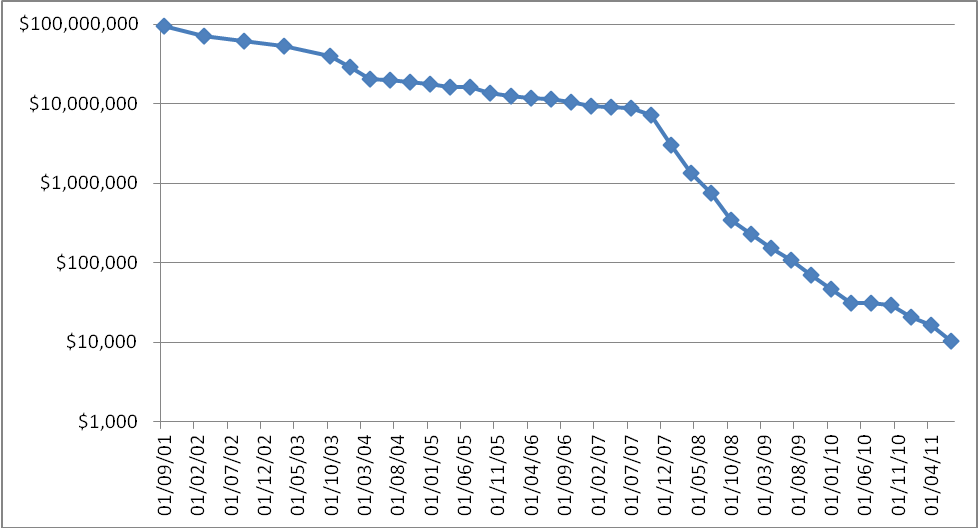
\includegraphics[scale=0.75]{cost.png}
\end{center}
\caption{Yıllara göre genom dizileme maliyetindeki değişimler. http://www.genome.gov/SequencingCosts/ adresinden alınmıştır.}
\label{fig:cost}
\end{figure}


Şu anda kullanılmakta olan birçok farklı ikinci ve üçüncü nesil YND platformu vardır. Bunların başlıcaları olarak 454 Life Sciences şirketinin ürettiği GS FLX sistemi, Illumina şirketinin ürettiği HiSeq2000/HiSeq2500/HiSeq3000/HiSeq4000, Ion Torrent'in PGM ve Proton, Pacific Biosciences'in SMRT teknolojisi ve PacBio RS platformu, Applied Biosystems'in SOLiD cihazı olarak listelenebilir. Çok daha yeni olarak nanoteknoloji temelli ``dördüncü nesil'' platformları (örn. Oxford Nanopore) piyasaya çıkmaya başlamıştır~\cite{Metzker2010,Loman2015}. Her ne kadar dizileme maliyeti çok düşmüşse de YND teknolojilerinin ürettiği verilerin bazı eksik yönleri vardır. Okunan ortalama dizi parçacığı uzunluğu çok kısa (örn. Illumina için 150 baz çifti), kullanılan DNA molekülleri çok küçük (örn. Illumina için 200-700 baz çifti), ve baz okuma hata oranı çok yüksek ve değişkendir (Illumina için \%0.1, Pacific Biosciences için \%15).


YND teknolojilerindeki baş döndürücü ilerleme, bu verilerin işlenmesine olan ihtiyaç nedeniyle bilgisayar bilimleri alanında da artan bir faaliyete neden olmuştur~\cite{Pop2008}. Elde edilen verilerin referans genomuyla karşılaştırılması ile değişik bireyler arasındaki genomik farklılıkların bulunması önemli bir araştırma alanıdır~\cite{Alkan2011,DePristo2011}. Bu nedenle 2.500 insan genomunun ayrıntılı incelenmesini amaçlayan 1000 Genom Projesi halen devam etmektedir~\cite{1000GP,1000GP2012}. Normal farklılıkların dışında genetik hastalıkların nedenlerinin bulunması için de YND platformları eşsiz bir güç sunmaktadır~\cite{Bamshad2011}. Ayrıca YND yöntemleri hücrelerdeki tüm RNA moleküllerinin tamamı anlamına gelen transkriptom dizilenmesi~\cite{Wang2009} ve genlerin aktivasyonlarini ölçmek~\cite{Park2009} için de kullanılabilir. 

Yukarıda belirtilenlerin dışında YND teknolojilerinin yoğunlukla uygulandığı bir alan da tüm genom dizileme birleştirmesi (de novo genome assembly) yoluyla farklı organizmaların referans genomlarının çıkarılmasıdır~\cite{Schatz2010}. Bugüne kadar geliştirilmiş olan genom birleştirme algoritmalarının hepsi çizge kuramı (graph theory) temellerine dayalı algoritmalardır. Başlıca iki tür genom birleştirme yöntemi vardır. Bunlardan ilki olan örtüşme çizgesi (overlap graph) yönteminde dizi parçaları çizgede uç olarak ifade edilir ve arasında başlangıç/sonuç ilişkisi olan dizi parçaları arasına kenar eklenir ve oluşan çizge üzerinde Hamilton turu (Hamiltonian path) aranır. Bu yöntemin örnekleri arasında eski nesil dizileme teknolojileri için kullanılan Celera Assembler~\cite{Myers2002}, Phusion~\cite{Mullikin2003} ve ARACHNE~\cite{Batzoglou2002} bulunur. İkinci ana yöntem genelde YND birleştirmelerinde kullanılan de Bruijn çizgesidir. Bu yöntemde YND dizi parçaları daha küçük ve aynı uzunlukta parçalara bölünür (k-mer), bu k-mer'ler çizgede uç olarak ifade edilip aynı dizi parçasından gelen k-mer'ler arasına kenar konulur. Bu şekilde oluşturulan çizgede Euler turu (Eulerian path) aranır. Bu yöntemi uygulayan başlıca birleştiriciler ise EULER~\cite{Chaisson2009}, ABySS~\cite{Simpson2009}, Velvet~\cite{Zerbino2008} ve SOAPdenovo'dur~\cite{Li2010b}. Yukarıda bahsedilen algoritmaların hepsi bir seferde sadece tek bir veri tipi kullanabilir, ve farklı verilerden ayrı ayrı oluşturulan farklı birleştirmeler daha sonra birbirlerine eklenir (iskeleleme/scaffolding).

Her ne kadar dizilemedeki ucuzlama nedeni ile arka arkaya bir çok hayvan ve bitki için referans genomu çıkarılıyorsa da bu referansların tamamlılık oranı ve kalitesi İnsan Genom Projesi~\cite{IHGSC2001} ile oluşturulan referans genomunun kalitesinin çok gerisinde kalmıştır~\cite{Schatz2010,Alkan2011c}. Yakın zamanda sadece YND kullanılarak oluşturulan yeni insan genomu birleştirme projelerindeki~\cite{Li2010b,Gnerre2011} hatalar ve eksiklikler genom birleştirme yöntemlerinin önünde alınması gereken çok yol olduğunu ortaya koymuştur~\cite{Alkan2011c}. En önemli eksiklikler birleştirilen genomların devamlı parça (contig) sayısının çok yüksek oluşu, tekrarlı ve duplike bölgelerin yanlış ya da eksik birleştirilmiş oluşudur~\cite{Alkan2011c}. Bir genom birleştirme projesinin en büyük amacı gen dizilerinin belirlenmesi iken, yukarıda bahsedilen sorunlar nedeniyle, bilinen genlerin YND kullanılarak yapılan birleştirmelerde bir çok parçaya ayrıldığı görülmüştür (Şekil~\ref{fig:shatter}). Bu nedenlerden dolayı, güvenilir ve doğru yeni genom birleştirme algoritmalarına ihtiyaç vardır.


\begin{figure}[htb]
\begin{center}
  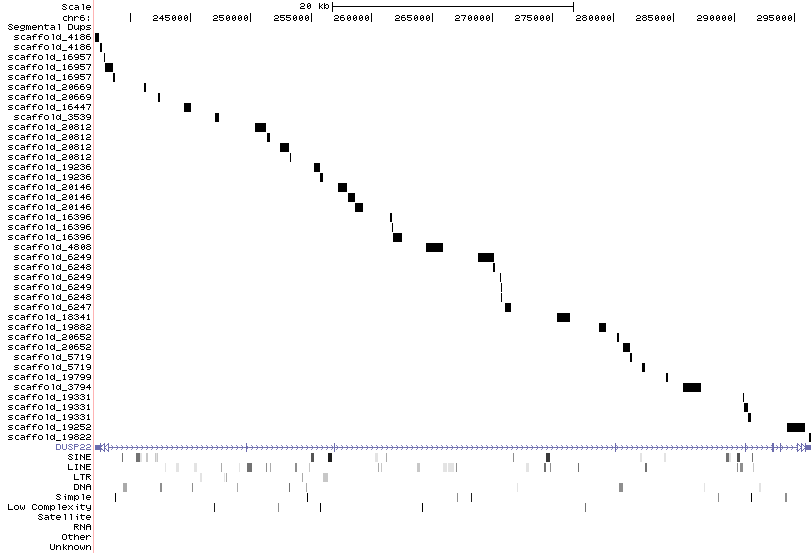
\includegraphics[scale=0.45]{shatter.png}
\end{center}
\caption{Sadece Illumina platformu kullanılarak yapılan bir tüm genom birleştirmesi~\cite{Li2010b} sonucunda ortaya çıkan referanstaki {\it DUSP22} geninin onlarca parçaya ayrıldığı görülmüştür~\cite{Alkan2011c}.}
\label{fig:shatter}
\end{figure}



Bunlara rağmen her YND teknolojisinin diğerlerine göre bazı avantajları vardır. Örneğin Illumina platformu en çok veriyi en ucuza üretebilir (10 günde 600 milyar baz çiftinden fazla) ve baz okuma hata oranı en azdır (\%0.1). 454 cihazı diğerlerine göre daha büyük molekülleri eşli dizileyebilir (yaklaşık 20.000 baz çifti). Pacific Biosciences ise şu anki teknolojiler arasında ürettiği ortalama dizi uzunluğu en fazla olan platformdur (1.4 kb) ve ``grup dizileme'' (strobe sequencing) teknolojisi ile eşli dizilemeye (paired-end sequencing) göre bir molekülden daha fazla bilgi çıkarabilir (Şekil~\ref{fig:strobe}). Bu nedenledir ki, aynı anda birden fazla teknoloji ile elde edilmiş verileri kullanmak, her bir teknolojinin diğerlerine üstün yanlarından faydalanıp, sahip olduğu dezavantajları da diğer teknolojilerin avantajları ile gidermek en uygunu olacaktır. Örneğin Illumina'nın sağladığı yüksek kalitedeki baz okuma doğruluğu ile Pacific Biosciences'ın \%15'lik hata oranını düzelterek, aynı zamanda Pacific Biosciences'in gruplu ve uzun dizileme özelliği sayesinde Illumina'nin kısa dizilerinin birleştirilmesini geliştirip tekrarlı alanlardaki yapısal birleştirme hatalarını en aza indirgemek mümkün olacaktır.

\begin{figure}[htb]
\begin{center}
  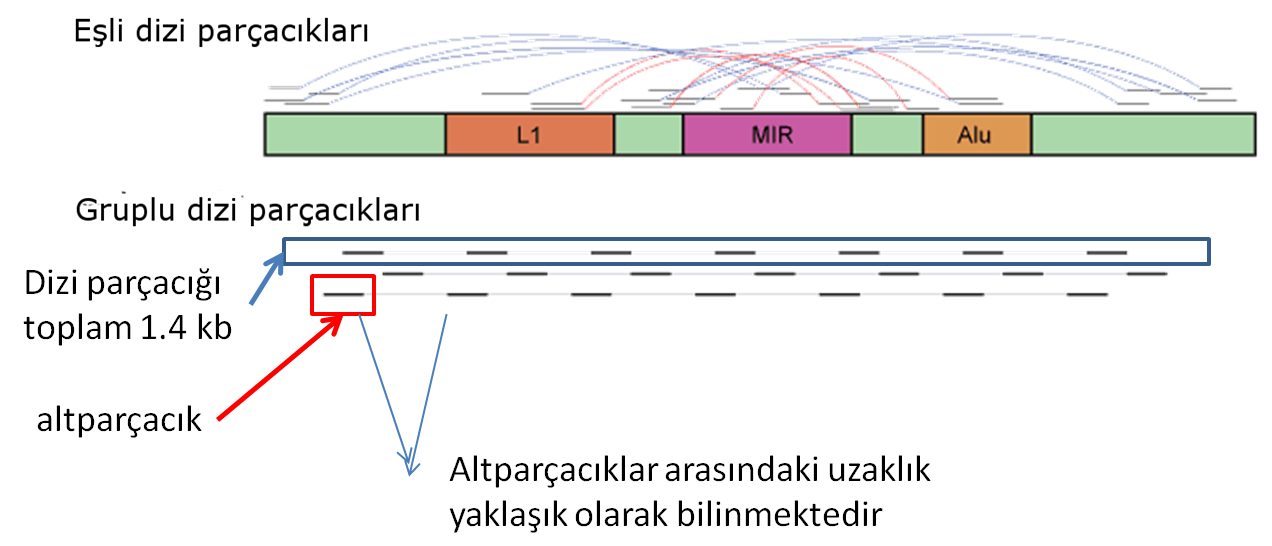
\includegraphics[scale=0.75]{strobe.png}
\end{center}
\caption{Eşli dizileme (paired-end sequencing) ve gruplu dizileme (strobe sequencing). Illumina, Ion Torrent, 454, Complete Genomics ve SOLiD cihazları ile eşli dizileme yapilabilinirken, Pacific Biosciences gruplu dizilemeyi desteklemektedir.}
\label{fig:strobe}
\end{figure}


\noindent

\clearpage
\begin{center}
{\bf \Large 2. LİTERATÜR ÖZETİ}
\end{center}
\addcontentsline{toc}{section}{2. LİTERATÜR ÖZETİ}




\begin{center}
{\bf \Large 3. GEREÇ VE YÖNTEM} 
\end{center}
\addcontentsline{toc}{section}{3. GEREÇ VE YÖNTEM}
\noindent

{\bf \large 3.1. Genel bakış ve özet}
\addcontentsline{toc}{subsection}{3.1. Genel bakış ve özet}

Bu projenin başvurusunda da kaba taslağını verdiğimiz aynı anda kısa ve uzun dizilerin kullanımına olanak sağlayacak birleştirme algoritmasının çalışmalarına başladık. Projenin bu aşamasında
 kısa diziler için Illumina ve uzun diziler için Pacific Biosciences (PacBio) verileri kullanacağız. Bu algoritmayı geliştirmek ve test etmek için 8 farklı BYK'den elde edilmiş 
hem Illumina hem de PacBio verilerini University of Washington'daki Evan Eichler'dan temin ettik. Bu verilerin içeriği ve Quiver 
programi kullanılarak birleştirilme sonuçları Şubat 2014’te Genome Research dergisinde yayınlanmıştır~\cite{Huddleston2014}. 

Tek veri tipini kullanan genom birleştirme algoritmaları teorik olarak her ne kadar iyi çalışsa da, gerçek verilerdeki karışıklıklar bu algoritmaları pratikte daha güçsüz kılmaktadır. Dolayısıyla, tasarlanan genom birleştirme algoritmalarının gerçek verilerinin getirdiği komplikasyonlara karşı dirençli (robust) olmaları gerekmektedir. Gerçek verilerin getirdiği komplikasyonlardan en önemlilerinden üç tanesi:

\begin{enumerate}
\item
  Yapısı gereği genom dizisi kendi içinde tekrarlanan diziler (repeat) içermektedir. Özellikle, bu tür tekrarlanan diziler kısa dizilerden daha uzun olduklarında, tekrar bölgelerine denk gelen kısa dizilerin aslında tekrar bölgelerinin hangisine denk geldiğini anlamak zor bir problem olmaktadır. İşleri daha da zorlaştıran başka bir nokta ise, ters çevrilmiş tekrarlanan diziler (inverted repeat), hatalı tekrarlanan diziler (inexact repeat), ve tekrarlanan dizilerin içinde başka tekrarlanan dizilerin yer alabiliyor olmasıdır. Tekrarlanan dizilerin çizge üzerinde bulunup oluşturdukları genom birleştirme sorunlarının çözülmesine ``tekrarların çözülmesi'' (repeat resolution) adı verilir, ve esasen genom birleştirme probleminin en zor aşamasını oluşturmaktadır.

\item
  Tekrarların çözülmesini daha da zorlaştıran bir başka nokta ise dizileme hatalarıdır (sequencing errors). Geliştirilen algoritmaların dizileme hatalarına toleranslı davranmaları bazen gerçekleşmemesi gereken birleşmelerin gerçekleşmelerini sağlayabilmektedir.

\item
  Üçüncü bir neden genomdaki ploitlik ve heterozigositedir. Farklı haplotiplerden gelen az miktarda farklılaşmış diziler genom birleştirme çizgesi üzerinde hatalı tekrar dizilere benzerlik gösterebilir.

\item
  Son olarak, genomun her kısmının aynı miktarda kısa dizilerle kapsanmadığını da işin içine dahil etmemiz gerekmektedir. Bu probleme ``eşit dağılmayan kapsama'' (non-uniform coverage) ismi verilir.

\end{enumerate}

Proje başvurusunda, Illumina cihazının \%0.01 hata payıyla ürettiği 100 baz çifti uzunluğundaki dizileri kullanarak, PacBio cihazının 10\%-15\% hata payıyla ürettiği 4000-5000 baz çifti uzunluğundaki dizilerin hata oranını düşürmeyi önermiştik. Bu probleme çözüm olarak farklı bir yöntemi geliştirmeye başladık. Problemi tekrarlayalım: 

{\bf Problem:}

İki farklı veri kaynağından elde edilen genom dizileri bulunmaktadır. PacBio'dan elde edilen dizi kümesini $P$, Illumina'dan elde edilen dizi kümesini ise $I$ diye adlandıralım. $P$ kümesi uzunlukları $n$ olan $N$ adet uzun diziden oluşmaktadır. $I$ kümesi ise uzunlukları $m$ olan $M$ adet kısa diziden oluşmaktadır. $I$ kümesindeki her dizi $P$ kümesinden sabit sayıda dizi ile hizalanacaktır (yani, Levenshtein mesafesi önceden belirlenen eşiğin altında olacaktır). Problem, $I$ kümesindeki her dizi için $P$ kümesindeki hizalanabilecek ``potansiyel'' dizileri hızlı ve verimli biçimde bulmaktır.

{\bf {\underline{Çözüm:}}}

İki dizinin birbirlerine benzeyip benzemediklerini ve dolayısıyla hizalanıp hizalanamayacaklarını belirlemek için bu iki dizi arasındaki Levenshtein mesafesine~\cite{Levenshtein1966} bakmak yeterlidir. Eğer Levenshtein mesafesi belirli bir eşiğin altındaysa iki dizi birbirlerine benziyorlar, veya eşiğin üstündeyse ise birbirlerinden farklılar denebilir. Ancak uzunlukları $m$ ve $n$ olan iki dizinin arasındaki Levenshtein mesafesini hesaplamak $O(nm)$ zaman karmaşıklığı gerektirmektedir. Locality-sensitive hashing (LSH) gibi olasılıklı yöntemler bizim problemimizde çalışmamaktadır,  çünkü PacBio'daki hatalar baz çiftlerinin eklenmesine veya silinmesine neden olmaktadır (indel) ve dolayısıyla LSH'in rastgele seçeceği baz çiftlerin sıraları değişmektedir.


LSH yönteminin Levenshtein uzaklığı için kullanılamaması sebebiyle, hizalanabilecek ``potansiyel'' dizi çiftlerinin arasındaki uzaklık için farklı bir metrik kullanmayı öneriyoruz. Bu metrik aynı zamanda LSH'in de uygulanabilmesini sağlaması gerekiyor. Literatürde LSH'in kullanılabilmesini sağlayan uzaklık metriklerine ``LSHable'' adı verilir. Bu özelliği sağlayan en kolay ve kullanışlı metrikleriden biri Jaccard benzerlik metriğidir. A ve B kümeleri arasındaki Jaccard metriği, iki kümenin kesişiminin boyutu ile iki kümenin birleşmesinin boyutu arasındaki orantıyı ölçmektedir.


Jaccard metriği için LSH'i literatürde var olan bir yöntemi \cite{Broder1998} kullanarak uygulayabiliriz. Burada, her diziyi temsil eden k-mer kümeleri oluşturulacaktır. Eğer iki dizinin k-mer kümeleri arasındaki Jaccard değeri yüksekse yüksek ihtimalle bu iki dizi birbirine hizalanacaktır diyebiliriz.

Anlattığımız yöntemin prototipini küçük veriler üzerinde deneyerek çalıştığını gözlemledik. Bundan sonraki adımda, Jaccard benzerliği üzerinden LSH kullanarak her kısa dizinin uzun diziler kümesindeki ``yaklaşık en yakın komşularını'' parallel hesaplayan algoritma geliştirmeye başladık. Bu algoritma, insan genomunun PacBio dizilerindeki hataları Illumina dizilerini kullanarak kabul edilebilir bir zamanda düzeltecektir.




{\bf \large 3.2. Havuzlanmış klon dizileme ile genom iskeleleme}
\addcontentsline{toc}{subsection}{3.2. Havuzlanmış klon dizileme ile genom iskeleleme}


Günümüzde yeni nesil dizileme (YND) teknolojilerinin yaygınlaşması ve dolayısıyla verilerin düşük maliyetlerde elde edilebilmesi, de novo (referans genom olmadan) 
genom dizilemeye olan ilgiyi artırdı.
Bu durum, kısa okumalardan (short reads) güvenilir ve yüksek kalitede taslak genoma olan ihtiyacı ortaya çıkardı. YND teknolojileriyle elde edilen milyonlarca okumalar ilk olarak bitişikler (contig) adı verilen DNA dizilerinin bulunmasında kullanıldı. Daha sonra bu bitişikler, iskeleleme algoritmalarıyla (scaffolding) birbirlerine olan uzaklıkları ve sıralamaları bulunarak iskeleler haline getirilebilir.

Prof. Evan Eichler ve Prof. Jay Shendure'den alınan ve NA12878 kodlu insan genom örneğinden elde edilen ``havuzlanmış'' (pooled) Bakteri Yapay Kromozomlarını~\cite{Kitzman2011} kullandık. 
(BYK; İngilizce Bacterial Artificial Chromosome). 
Amacımız tüm genomu kapsayacak sayıda üretilip Illumina ile dizilenmiş BYK klonlarını kullanarak bir insan tüm genom dizisinin düzeltilmesi ve geliştirilmesidir.
	
Bu BYK’ların uzunluğu yaklaşık 150.000 – 200.000 baz çiftidir. İlk olarak bu BYK'lardan rastgele seçilen 288 bakteri yapay kromozomu havuzu oluşturuldu. Her havuzda genomun yaklaşık \%3'ünün 
kapsanması hedeflendi. Buradaki amaç rastgeleliği arttırarak, duplikasyonlardan kaynaklanan olası yanlış eşleşmelerin mümkün olduğu kadar önüne geçebilmektir. 
Duplikasyonlar \%90 oranında benzeyen dizi parçalarıdır. 

BYK’lar haricinde aynı insanın tüm genomundan elde edilmiş DNA dizileri (WGS) daha önce Broad Enstitüsü’ndeki araştırmacılar tarafından ALLPATHS~\cite{Gnerre2011} programı kullanılarak birleştirilmiş, ve bu birleştirme sonuçları tüm araştırmacıların kullanımına açılmıştır. Ancak bu projenin başvuru amaçlarında da belirtildiği üzere, bu birleştirme sonucunda edilen bitişiklerde gerek gen ve ekzonların temsili, gerekse tekrarlı DNA dizileri nedeniyle parçalanmalar ve yanlış birleştirmeler bulunmaktadır~\cite{Alkan2011c}. Gene projenin başvuru amaçlarında belirtildiği üzere, tüm genom dizileme ve birleştirme verilerini diğer şekillerde elde edilmiş veriler ile birlikte kullanmayı amaçladığımızdan bu veriyi de NCBI internet sayfasından indirdik.

ABySS~\cite{Simpson2009}, ALLPATHS~\cite{Simpson2009}, ya da diğer genom birleştirme algoritmalarının oluşturduğu iskeleler tam olarak optimize edilmemiştir. Dahası, elimizdeki BYK tabanlı veriler de tüm genom dizilemeden farklı olduğu için, bu veriler doğrudan genom birleştirme araçlarına yüklenemez. Bundaki sebep, tüm genom dizilemelerinin tamamen rastgele olarak üretilmiş olması, havuzlanmış BYK verilerinin ise daha hiyerarşik bir yapıda oluşturulmuş olmasıdır. Bu nedenle ilk aşama olarak literatürde tanımlanmış iskeleleme algoritmalarının bir tetkikini yaptık. Buradaki amaçlarımız, bu araçların elimizdeki veriler ile uyumluluğunu test etmek, ve aynı zamanda eksikliklerini sınıflandırmaktır.

İskelelerin bulunması (Şekil~\ref{fig:scaffold} NP-zor (NP-hard) bir problem olduğu için geliştirilen iskeleleme (scaffolding) araçları keşifsel (heuristic) yöntemlerle yaklaşık sonuçlar üretebilmektedir. Bu dönem yaptığımız çalışmalarda geliştirilmiş iskeleleme araçlarından elimizdeki veri türlerine uygun olan 5 aracı çalıştırmayı hedefledik. Diğer kromozomlara kıyasla boyu daha kısa olan kromozom 20'nin iskelelerini bulmaya çalıştık. Kod adı NA12878 olarak bildiğimiz bireyin kromozom 20 verisinin, hem tüm genom (whole genome shotgun (WGS)) yöntemi hem de bakteri yapay kromozomları (BAC) dizileme yöntemiyle elde edilmiş verileri bulunmaktaydı. Öncelikle ALLPATHS~\cite{Gnerre2011} birleştirme programı kullanılarak WGS okumaları (read) bitişikler haline getirildi. Kromozom 20 datasından ALLPATHS kullanılarak hesaplanan 250 bitişik elde edildi. Bu bitişiklerleri elimizdeki 288 BAC ve 96 fozmid havuzları ile iskeleler haline getirmek için farklı iskeleleme araçları kullandık ve performans, elde edilen iskelelemelerin kalitesi, elde edilen iskelelemelerin N50 değerleri (bitişik uzunlukları azalan bir şekilde eklendiği zaman genom büyüklüğünün yarısına erişildiğinde en son eklenen bitişiğin uzunluğu), bulunan en uzun iskelenin boyu ve iskeleleme sayılarına bakarak en iyi iskeleleme aracını bulmaya çalıştık. 

\begin{figure}[htb]
\begin{center}
  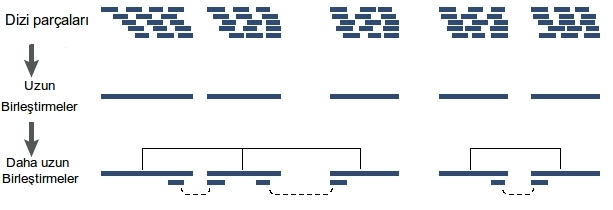
\includegraphics[scale=0.75]{scaffold.png}
\end{center}
\caption{Dizi parçalarından bitişiklerin ve iskelelerin elde edilmesi.}
\label{fig:scaffold}
\end{figure}


Çalıştırdığımız iskeleleme araçları kısaca şunlardır:

\begin{enumerate}

\item Phrap~\cite{phrap}: Önce WGS verileriyle ALLPATHS~\cite{Gnerre2011} kullanarak elde edilen bitişikleri ABySS~\cite{Simpson2009} programı kullanılarak birleştirilmiş BYK'lar ile geliştirip iskeleleri bulmaya çalıştık. Ancak tek bir havuzdan gelen verileri birleştirmek bile  3 günden daha uzun sürdüğünden ve toplam $288 + 96$ havuz düşünüldüğünde, bu yaklaşımın etkin bir çözüm olmayacağına karar verip bu iskeleleme aracından vazgeçtik.
  
\item ALLPATHS~\cite{Gnerre2011} programı ile birleştirilip contig haline gelen verilerimiz, SCARPA~\cite{Donmez2013}, OPERA~\cite{Gao2011}, SSPACE~\cite{Boetzer2011}, ve BESST~\cite{Sahlin2014} iskeleleme araçlarıyla çalıştırılarak iskelelemeler haline getirilip sonuçlar alındı. (Bulgular). 
  
  \begin{enumerate}
    \item
      SSPACE: Geliştirilmiş ilk iskeleleme programlarından biridir~\cite{Boetzer2011}. Fırsatçı (greedy) bir algoritma ile, ilk olarak en optimal bitişikleri birleştirir ve bu iskeleleri sonraki okumalar ile genişleterek ilerler. Buradaki en büyük dezavantaj, iskeleleme sırasında en olası görünen birleştirmenin, daha sonraki aşamalarda yanlış iskelelemelere sebep olmasıdır. İşletim anında en uygun görünen birleştirme yanlış sonuçlara sebep olabildiği için çizge tabanlı algoritmaların doğruluk oranının daha yüksek olduğu düşünülmüştür. 

    \item OPERA: İskeleleme probleminin NP-zor bir problem olduğu gösterildikten sonra bu problemi optimal çözebilmek için belirli  kısıtlayıcı parametreler ile çözmeye çalışmıştır~\cite{Gao2011}. İskeleleme işleminin her bir aşaması için alt ve üst sınırlar belirler ve bir sınır içerisinde problemi çözer. İskeleleme işleminden önce veriyi ön işleme ile yanlış Iskeleleme işlemine sebep olacak  tutarsız verilerden temizler.
      
    \item SCARPA: Lineer programlama ile optimal iskeleleri bulmayı amaçlar~\cite{Donmez2013}. Aracın yazarları diğer iskeleleme programlarındaki kayıp birleştirmeleri farkedip bu probleme özel algoritma geliştirdiklerini iddia etseler de, sonuçta yine kayıp birleştirmeler olmuştur.
      
\item BESST: Diğer iskeleleme programlarının bitişikler arası boşluk uzunluğunu yanlış bulduklarını gösterip, buna özel algoritma geliştirmişlerdir~\cite{Sahlin2014}. Diğer üç program ile karşılaştırıldığında, en çok bitişiği en az iskeleye indirebilmiştir. Ancak veri kaybı oldukça fazladır.
  \end{enumerate}

\end{enumerate}

Bu programların en önemli dezavantajı veri kaybının olmasıdır. İskeleleme işlemi sonucunda, bitişiklerin yön ve sıralamasının bulunması, aralarındaki uzaklıkların ``N'' 
karakterleriyle doldurulması sonucu uzunluklarının artması beklenirken, dört programda da sonuç uzunluk azalması olmuştur. Bunun başlıca sebebi, birleştirilemeyen veya oryantasyonu bulunamayan bitişiklerin çalıştırılan programlar tarafından elenmesidir.

Sonuç olarak, farklı iskeleleme programları, parametreleri, hizalama yöntemleri ve ürettikleri iskeleler test edilip farklılıklar tespit edilmiştir ve yeni tasarlanılacak iskeleleme programının geliştirilmesi için gereklilikler ve oluşabilecek hatalar not edilmiştir.

\clearpage
{\bf \large 3.3. Birden fazla platform verisi ile genom birleştirmelerde hata düzeltimi}
\addcontentsline{toc}{subsection}{3.3. Birden fazla platform verisi ile genom birleştirmelerde hata düzeltimi}


Daha önceki bir çalışma için insan genomuna ait 13. kromozom bir BAC'ın (Bacterial Artificial Chromosome) içine halihazırda klonlanmıştı. 
Bu BAC klonunu Illumina, Roche/454 ve Ion-Torrent platformlarında ayrı ayrı diziledik (Tablo \ref{tab:dataprop}).
Mira~\cite{Chevreux1999} birleştiricisiyle (assembler) şablona dayalı birleştirme yöntem kullanarak Roche/454 okumalarıyla (read), ``altın standart'' bir referans dizisi elde ettik. Bu ``altın standart'' referans dizisini Illumina okumalarıyla düzelttik.
Roche/454 ve Ion-Torrent platformları benzer dizileme sapmalarına (Örn. problemli homopolimerler) sahip olduklarından, bu çalışmayı iki ayrı gruba böldük: Illumina \& Roche/454 and Illumina \& Ion-Torrent. Böylelikle Roche/454 ve Ion-Torrent verisini kontrol etme imkanı bulmuş olduk.

\begin{table}[htb]
\begin{tabular}{|l|l|l|l|l|}
\hline
Teknoloji & Uzunluk aralığı & Ortalama uzunluk & Ortalama baz kalitesi (phred) & Tür \\ 
\hline
Illumina & 101bp & 101bp & 38 & eşli \\
Roche/454 & 40bp-1027bp & 650bp & 28 & tekli \\
Ion-Torrent & 5bp-201bp & 127bp & 24 & tekli \\
\hline
\end{tabular}
\caption{Veri özellikleri.}     
\label{tab:dataprop}
\end{table}


\paragraph{Ön işleme} 
Öncelikle düşük ortalama kaliteye (phred skor 17, veya $\geq$2\% hata oranı) sahip okumaları eledik. Daha sonra yüksek `N' yoğunluğuna (okumanın içerdiği N oranı \%$>$10) sahip okumaları çıkardık. Üçüncü olarak bazı bölgelerinde (genellikle başlangıç ve bitiş) düzensiz (non-uniform) baz dağılımı gösteren okumaların bu bölgelerini kırptık. Son olarak, birleştiricinin (assembler) ön işleme yöntemlerini kaçınılmaz olarak uyguladık.

\paragraph{Birleştirme} Birden fazla birleştirme aracı kullandık: kısa okumaları birleştirmek için de Bruijn çizge tabanlı bir birleştirici: Velvet~\cite{Zerbino2008}; ve uzun okumalardan oluşan veri guruplarını (Roche/454 ve Ion-Torrent) ayrı ayrı birleştirmek için iki farklı ``overlap-layout-consensus'' (OLC) birleştirici: Celera~\cite{Myers2000}, ve SGA~\cite{Simpson2012}. Ek olarak, uzun okumalar üzerinde bir de Bruijn çizge tabanlı birleştirici de kullanıldı, SPAdes~\cite{Bankevich2012}. Daha sonra klonlama işleminden kaynaklı kontaminasyonları belirlemek ve onlardan kurtulmak için tüm taslak birleştirmeler BLAST~\cite{Altschul1990} ile E.coli referans genomuna hizalandı. En sonunda $1$ kısa $3$ de uzun okuma birleştirmesi elde ettik.
 
\paragraph{Doğrulama} 
Kısa okumalardan elde edilen birleştirmeleri uzun okumaların birleştirilmesiyle elde edilen dizilere hizalamak için BLAST~\cite{Altschul1990} kullandık.
BLAST tekrarlardan dolayı birden fazla hizlama lokasyonu raporladığından, sadece ``en iyi'' eşleşme lokasyonları kabul edildi.
Kısa okumalar daha az dizileme hatası içerdiğinden, aralarında anlaşmazlık görüldüğünde kısa okumalara dayanan birleştirmenin raporladığı diziyi uzun okumalardan elde edilen birleştirmenin raporladığına tercih ettik.
Bunu yaparak, daha ``az parçalı'' uzun birleştirmeler elde ettik. Şekil \ref{correction} uzun okumaların birleştirmelerinin hangi stratejiyle düzeltildiğinin görsel anlatımını temsil ediyor. 
Uyguladığımız strateji şu şekilde işliyor: Eğer kısa okuma birleştirmesiyle uzun okuma birleştirmesi arasında bir eşleşme varsa ve eşleşme uzun okuma birleştirmesinin başından başlamıyorsa, uzun okuma birleştirmesinin baş kısmını ekliyoruz.
Aynı zamanda eğer eşleşme kısa okuma birleştirmesinin başından başlamıyorsa (çok nadir bir durum) kısa okuma birleştirmesinin baş kısmını da küçük harflerle ekliyoruz. 
Kısa okuma birleştirmesinin ve uzun okuma birleştirmesinin eşleştiği bölgelerde kısa okuma birleştirmesini tercih ediyoruz. 
Eğer eşleşme kısa okuma birleştirmesinin sonunda bitmiyorsa (nadir), kısa okuma birleştirmesinin eşleşmeyen son kısmını küçük harflerle ekliyoruz.
Sonuç birleştirmesinin sürekliliğinin bozulacağı söylenebilir, ama bu tarz durumlarla çok seyrek karşılaşıyoruz.
Küçük harfler kullanmamızın sebebi o bölgede kısa okuma birleştirmeleriyle uzun okuma birleştirmeleri arasında bir anlaşmazlık olduğunu takip etmek istememiz, böylece bu bölgede baz kalitesi dizinin diğer bölgelerine göre daha düşük olacaktır.
Son olarak, uzun okuma birleştirmesinin eşleşmeyen son kısmını da ekleyip doğrulanmış birleştirme dizisini elde ediyoruz.  

\paragraph{Değerlendirme}
Her doğrulanmış birleştirmeyi ``altın standart'' referans dizisine  hizaladık, karşılaştırmaya dayalı değişik istatistikler hesapladık ve birleştirme kalitelerini değerlendirdik.
Aynı zamanda Illumina \& 454 ve Illumina \& Ion-Torrent verisiyle birlikte iki hibrid birleştirici, Celera-CABOG~\cite{Miller2008} ve Masurca~\cite{Zimin2013}, çalıştırdık ve bizim doğrulama metodlarımızdan elde ettiğimiz sonuçlarla bu hibrid birleştiricilerden elde ettiğimiz sonuçları karşılaştırdık.

\begin{figure}[htbp]
\begin{center}
  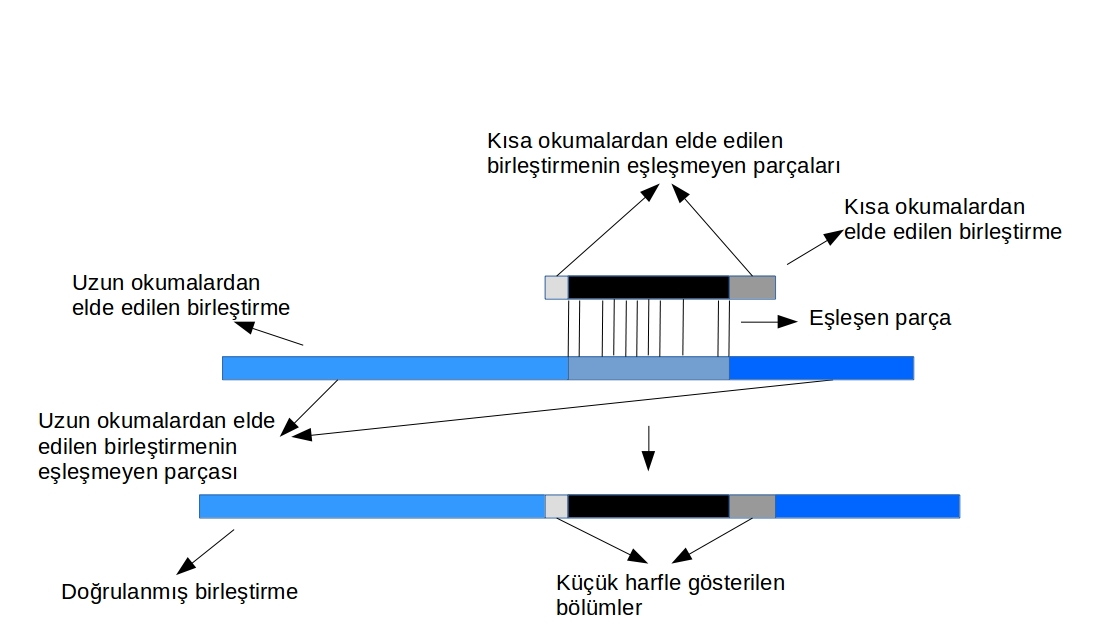
\includegraphics[width=14cm, height=8cm]{BACAlgorithmTurkce.jpg}
\end{center}
  \caption{Doğrulama metodu: Uzun okuma birleştirmelerini kısa okuma birleştirmelerinin hizalama bilgilerine göre doğrula.}
  \label{correction}
\end{figure}









\clearpage

{\bf \large 3.4. Illumina ve PacBio verilerini kullanan hibrit birleştirme algoritması}
\addcontentsline{toc}{subsection}{3.4. Illumina ve PacBio verilerini kullanan hibrit birleştirme algoritması}


{\bf 3.4.1. Hızlı Illumina-PacBio hizalanması için filtreleme}
\addcontentsline{toc}{subsubsection}{3.4.1. Hızlı Illumina-PacBio hizalanması için filtreleme}



PacBio'nun ilerde sunacağı iyileştirmelerin daha yüksek kalitede okumalar üretmeye başlayacağını varsaysak dahi genom birleştirme süreci üretilen parçaların teker teker bütün karşılaştırma kombinasyonlarını deneyeceğinden dolayı işlemcinin \%95 toplam çalışma süresini kapsamaktadır \cite{Berlin2015}. Bizim çalışmamızda, genom birleşimi yapmak için gereken kısa ve uzun dizilim parçalarının karşılaştırma sayısını azaltmayı amaçlayan bir çözüm öneriyoruz. Bunun için yöntemimiz ise seçilen filtrelerle gereksiz olması muhtemel karşılaştırmaları elemektir. Bunun yanında, uzun parçalardaki hata payını düşürmek için ise Illumina tarafından üretilen kısa parçalar ile PacBio tarafından üretilen uzun parçaları birbirleriyle karşılaştırıyoruz.

\paragraph{Problem Tanımı.}

Gelecek kuşak dizileme teknolojileri bütün bir genom dizilimini oluşturamadığından dolayı, bütün bir genomu yaratabilmek için üretilen parçalar arasındaki çakışmaların bulunması gerekiyor. Bu çakışma noktaları, iki parça arasında bir skor belirlemek için tanımlanıyor \cite{Staden1980}. İki parça arasında en yüksek skor bulunduğu zaman, iki parçayı düzgün bir pozisyonda hizalamak mümkün olabilir \cite{Staden1980}. Smith-Waterman (SW) dinamik programlama metodu, parçalar arasında hizalandırma yapmak için bilinen en hızlı metottur \cite{Smith1981}. $L$ uzunluğunda iki parçayı hizalandırmak için, SW metodunun hesapsal karmaşıklığı O($L^2$) olarak belirlenmiştir \cite{Smith1981}. Bundan dolayı, eğer toplamda $N$ sayıda ve her biri $L$ uzunluğunda parçalara sahipsek, bütün hizalandırmaları bulmanın hesapsal karmaşıklığı O($N^2$$L^2$) olacaktır.

Belirtilen bu hesapsal karmaşıklık şu anki gelecek kuşak dizileme teknolojilerini üzerinde uygulanabilir düzeyde değildir. Yukarıda belirtilen hesapsal karmaşıklıktan dolayı Illumina ile üretilen parçaları hizalandırmak çok yüksek miktarda bir hesaplama gerektirecektir bunun nedeni ise Illumina'nın ortalama olarak 1 ile 3 milyar arasında parça üretiyor olmasıdır \cite{Metzker2010}. Bu hesapsal karmaşıklığın oluşmasında dikkat edilmesi gereken iki husus vardır. Birincisi, bir parçayı diğer bütün $N$ adet parça ile karşılaştırdığımızdan dolayı ortaya çıkan $N^2$ adet karmaşıklık. Bir diğeri ise $L$ uzunluğunda bir parçanın diğer $L$ uzunluğunda bir parçayla her bir karakterinin teker teker karşılaştırmasından ortaya çıkan $L^2$ karmaşıklıktır. Bundan dolayı, hesapsal karmaşıklığı düşürebilmek için hem karakter ölçeğinde hem de parçalar arasındaki karşılaştırmalardan teker teker bütün kombinasyonları denemeye gerek duymayan bir yöntem önermemiz gerekiyor. Eğer en fazla $L$ uzunluğunda olan $N$ adet parçayı teker teker karşılaştırmaya gerek duymadan hizalandırmanın mümkün olduğunu kanıtlayabilirsek, SW metodunun hesapsal karmaşıklığını da böylece düşürebilmiş oluruz.

Bunun yanında, PacBio tarafından üretilen parçaların hata oranının, Illumina tarafından üretilen parçalara kıyasla çok daha yüksek olduğunu belirtmiştik. PacBio için hata oranı \%14 \cite{pacbioerr} ve Illumina parçaları için ise hata oranı \%0.1 - \%1 civarındadır \cite{Lou2013}. Ancak belirttiğimiz gibi Illumina tarafından üretilen parçalar 10 ile 100 katı kadar oranda PacBio parçalarına kıyasla daha küçük olduğu için Illumina ile yineleyen parçalar elde etme olasılığı artmaktadır. Bundan dolayı, güncel gelecek kuşak dizileme teknolojileri için hem en az 10000 baz çifti uzunluğunda hem de çok düşük hata payı oranında parçalar üretmek mümkün değildir. Eğer böyle bir teknolojiye sahip olunsaydı çok daha az yineleyen parçalara sahip olunacağı için, bu durum tüm bir genomu tekrar birleştirme noktasında daha düşük bir hesapsal karmaşıklığa gerek duyardı. 

\paragraph{İlgili Çalışmalar.}

Lander-Waterman modeli genom birleştirme yöntemleri içinde en sık kullanılanlardan biridir \cite{Lander1988}. Bu model minimum coverage hakkında tahminleri toplamak için kullanışlı \cite{Lee2014}. Ancak, Lander-Waterman modeli genomda tekrarlayan dizilerin çok sıklıkla var olmadığını varsaydığı için, model tarafından elde edilen tahminler yeteri kadar güçlü veriler olmuyor. Bunun sebebi ise günümüz gelecek kuşak dizileme teknolojilerinin tekrarlayan parça boyutları özellikle 1000 baz çiftinden kısa olmaya başladığı zaman yüksek miktarda tekrarlayan parçalar üretme olasılığıdır.

Lee, Hayan ve ark \cite{Lee2014} tarafından geliştirilen hata düzeltme modelinde izlenen yöntem ise kısa parçaların uzun parçalar üzerinde hizalandırılması üzerine kuruludur. Yukarıda da belirttiğimiz gibi, uzun parçaların tekrarlayan kopyalarının oluşma olasılığı daha düşük olduğundan ve toplam parça sayısı daha az olacağından dolayı hesapsal karmaşıklığı iyileştirmek adına daha uzun parçaların kullanımı tercih edilir. Lee, Hayan ve ark önerdikleri modelde kısa parçaların kullanımını hizalama aşamasında destekleyici bir yapı şeklinde kullanıyorlar. Uzun parçalar üzerinde birleştirilen kısa parçaların, PacBio tarafından üretilen uzun parçaları kullanarak yapılacak genom birleştirme sürecinde bir yarar sağlayacağını savunuyorlar. \cite{Lee2014}. Bu kısa parçaların birleştirme işleminden sonra PacBio tarafından üretilen uzun parçalar üzerinde, kısa parçalar referans alınarak bir hata düzeltme işlemi yaptıklarını belirtiyorlar. Bu hata düzeltme işleminden sonra her ne kadar PacBio parçaları daha az hata barındırarak kullanılabilecek olsa da, Lee, Hayan ve ark SW metodunun hesapsal karmaşıklığındaki üst sınırda herhangi bir iyileştirme sunmuyorlar.

Berlin, Konstantin ve Ark ise genom birleştirme sürecindeki hesapsal karmaşıklığı düşürmek adına MinHash birleştirme modelini öneriyorlar \cite{Berlin2015}. Önerdikleri modelde bütün parçaların birbirleriyle karşılaştırılmasını önleyecek bir çözüm sunduklarını belirtiyorlar. Bütün parçaları veya parçaların daha ufak parçalarını indeksleme yöntemiyle sayılardan oluşan parmak izlerini yarattıktan sonra parçaların kendileri yerine bu sayıları karşılaştırma esnasında kullanıyorlar. Böylece karşılaştırma esnasında daha az işlem gücü harcayacak bir yöntem ve uyguladıkları filtrelerle genom birleştirme işlemini $N$ sayıda ve $L$ uzunluğunda parçalar için O($N$$L$) karmaşıklıkta tamamlayabiliyorlar \cite{Berlin2015}. Ancak bütün parçaların $L$ uzunluğunda olacağı varsayımı her zaman uygulanabilir bir varsayım olmayabiliyor. Eğer sadece uzun parçaların genom birleştirme işleminde kullanıldığını belirtmiş olursak, bu varsayım muhtemelen uygulanabilir bir varsayım olabilir. Ancak daha önceden de belirttiğimiz gibi, kısa parçaların uzun parçalar üzerinde hata düzeltme amacında kullanılması genom birleştirme işleminden önce yapılabilecek işlemlerden biridir. Bundan dolayı hem hata oranını düşürmek hem de hesapsal karmaşıklığı düşürmek, bütün parçaların $L$ uzunluğunda olması gerekliliğinden mümkün olamamaktadır.

\paragraph{Amaç.}

PacBio tarafından üretilen uzun parçaların ve Illumina tarafından üretilen kısa parçaların kullanımında ne gibi avantajların ve dezavantajların olabileceğini sıklıkla dile getirdik. Açıkça görülebiliyor ki eğer PacBio uzun parçalar üretirken aynı zamanda Illumina'nın sunduğu hata oranında ve maliyette bu parçaları üretebiliyor olsaydı, PacBio, Illumina karşısında daha tercih edilebilir durumda olurdu. Bundan dolayı, Illumina hala market lideri konumunu korumaktadır. Ancak, her iki teknolojinin de bize sunduğu avantajlardan bir hibrit model içinde faydalanmalıyız. Bundan dolayı, ilk amacımız Illumina tarafından üretilen kısa parçaları kullanarak PacBio'nun uzun parçalarının hata oranını düşürmek. Bu şekilde uzun parçaları daha az hata oranıyla kullanabiliyor olacağız.

SW metodunun optimal düzeyde hizalandırma yapabilmesi için gereken hesapsal karmaşıklığı belirtmiştik. Şu anlaşılıyor olmalıdır ki; SW metodunun her ne kadar optimal düzeyde hizalandırma yapmayı başarabilse de elimizde çok fazla sayıda (örneğin milyarlarca) parça olduğu zaman hesapsal karmaşıklığı bu milyarlarca adet parça üzerinde ölçeklenebilir bir boyutta olamıyor. Bundan dolayı büyük genomları tekrar birleştirme aşamasında hesapsal karmaşıklık düzeyi ve ne kadar hassas düzeyde birleştirme yapıldığı arasında bir dengeleme yapmak gerekiyor. Şu anki aşamada en düşük hesapsal karmaşıklık ile en hassas şekilde birleştirme işlemi yapmak belirttiğimiz gibi ölçeklenebilir bir boyutta olmamaktadır. Bundan dolayı ikinci amacımız ise her bir parçanın diğer bütün parçalarla kıyaslanmasını önleyecek bir yöntem geliştirmek. Bu yöntemde hesapsal karmaşıklığı düşürebilmek adına hassaslık seviyesinde yaşayabileceğimiz bazı kayıpları tolera edebiliriz.


\paragraph{Hata oranının düşürülmesi.}
Amacımız, PacBio tarafından üretilen parçaların hata oranını düşürmek olduğundan dolayı, kısa parçaları bu amaç için kullanıyor olacağız. $N_i$ adet ve $L_i$ uzunluğunda, Illumina/Solexa gelecek kuşak dizileme makinası tarafından üretilen parçalarımız var. Aynı zamanda, $N_p$ adet ve $L_p$ uzunluğunda PacBio'nun SMRT makinası tarafından üretilen parçalarımız var. Aynı genom için, Illumina'yı $n_i$ kez çalıştırıyoruz. Eğer her kısa parçanın, $S_{i,i}$, uzun parça(lar), $S_{p,i}$, üzerinde belli pozisyon(lar)a hizalandığını düşünürsek, $j$'inci uzun parça ve $k$ pozisyonu için hizalanan kısa parçaların kümesi aşağıdaki gibi tanımlanabilir:

\begin{equation} \label{eqn:seqset}
\forall j \in \{1,2, \dots, N_p\} \hspace{0.3cm} ve \hspace{0.3cm}  0 \leq n \leq N_i \hspace{1cm}  f(S_{p,j}, k) = < S_{i,k_1},  S_i,k_2 , \dots, S_{i,k_n} >
\end{equation}

Böylece $S_{p,j}$ parçasının $k$ pozisyonundaki karakterini, Denklem~\ref{eqn:seqset}'de belirtilen kümenin içinde yer alan kısa parçaların o karakter üzerinde hizalanmış karakteriyle karşılaştırabiliriz. Eğer kısa parçaların çoğunluğu $k$ pozisyonunda farklı bir karakter olması gerektiğini gösteriyorsa, bu karakteri belirtildiği şekilde düzeltiriz. Illumina tarafından üretilen parçalardaki hata oranının PacBio tarafından üretilen parçalara kıyasla çok daha düşük olduğunu bildiğimizden dolayı, bu karakter düzeltmeleri çoğunlukla PacBio parçalarının hata oranını düşürecek yönde olacaktır.

\paragraph{Hesapsal karmaşıklığı azaltmak}
Hata oranını düşürmeden önce çözülmesi gereken problem ise hesapsal karmaşıklığın düşürülmesidir. Denklem~\ref{eqn:seqset}'de tanımlanan kümeyi oluşturabilmek için etkili bir yöntem önerebilmemiz gerekmektedir. Yöntemimiz, Berlin ve ark tarafından bahsedilen indeksleme yönteminden faydalanmaktadır \cite{Berlin2015}. Toplamda yapılan karşılaştırma sayısını azaltmak için iki adet filtre uyguladıklarını belirtiyorlar. $L$ uzunluğunda parçalar üzerinde bu filtreleri uyguladıkları için kısa parça ve uzun parçayı bir arada kullanmak için bu filtrelerin uygulanabilir olmadığını belirtmiştik. Bundan dolayı öncelikle uzun parçaları, kısa parçaların uzunluğu kadar bölümlere bölüyoruz. Dolayısıyla toplam parça sayısını en az $L_p / L_i$ katı kadar arttırmış oluyoruz. Eğer $S_{p,k}$ PacBio parçasını $l$ uzunlukta artışlarla bölümlere ayıracak olursan, toplam elde edilen bölüm sayısını şu şekilde tanımlayabiliriz:
\begin{gather*}
P_k = ((|S_{p,k}| - |S_{i,k}| )/l) + 1
\end{gather*}
Uzun parçaların kendi aralarında ve kısa parçaların da kendi aralarında ortalama bir uzunluğu olduğunu göz önünde bulundurursak, ortalama bir $P$ değeri belirtmemiz de mümkün olabilir bu sayede. Böylece SW metodu için hesapsal karmaşıklığımız O($P$$N_i$|$S_i|^2$) şeklinde tanımlanabilir. Fingerprint şeklinde adlandırılan ve verilen bir girdiye özel olarak sayısal bir değer veren fonksiyon ile beraber MinHash indeksleme fonksiyonlarının kullanımını içeren iki adet filtreleme uyguluyoruz. Fingerprint fonksiyonunu ve Minhash fonksiyonunu kullanmadan önce bütün kısa ve uzun parçaların k-merlerini yaratıyoruz. Sırasıyla kısa ve uzun parçaların k-mer kümelerini ise $K_{i,j}$ ve $K_{p,j}$ şeklinde tanımlıyoruz. Bu kümelerin boyutu ise
\begin{gather*}
| K_{(p | i), j} | = |S_{(p | i),j}| - k + 1
\end{gather*}
şeklinde tanımlanabilir. K-merleri fingerprint fonksiyonlarına sokmak için öncelikle pozitif bir $H$ değeri belirliyoruz. $H$ değeri, her bir k-meri kaç defa fingerprint fonksiyonuna soktuğumuzu belirtiyor. Fingerprint fonksiyonunu bütün k-merler için bir defa çalıştırdıktan sonra, bir sonraki çalıştırma esnasında aynı k-mer için farklı değer üretildiğinden emin olabilmek için önceki çalıştırmalarda verilmeyen bir besleme değeri veriyoruz. Bütün parçaların k-merlerini $H$ defa fingerprint fonksiyonuna soktuğumuzu düşünürsek, bu işlemi yapmanın hesapsal karmaşıklığı O(|$K$|$NH$) şeklinde belirtilebilir. Bu aşamadan sonra fingerprint fonksiyonlarından üretilen sayısal değerlere bakaram min-meri buluyoruz. Min-mer olarak belirtilen değer, $h$'inci fingerprint fonksiyonunun çalıştırılması esnasında en düşük positif fingerprint değerinin atandığı k-mere denk gelmektedir. Bütün min-mer değerlerini $sketch$ adı verilen bir dizide tutuyoruz. Açıkça görülebileceği gibi, her bir parça için $H$ adet fingerprint değeri üretildiği için, bu dizinin büyüklüğü de $H$ kadardır. Min-mer değerleri $sketch$ içinde toplandıktan sonra, iki parça arasındaki benzerliği Jaccard benzerliği \cite{Jaccard1901} hesaplamasıyla buluyoruz. Bizim durumumuzda iki parça sırasıyla kısa ve uzun parçalar olmak üzere $S_{i,m}$, $S_{p,n}$ şeklinde isimlendirilebilir. Berlin ve ark $h$'inci fingerprint fonksiyonu kullanılarak oluşan kümelerden iki parçanın benzerliğini
\begin{equation}
J(S_{i,m}, S_{p,n}) = \dfrac{|\Gamma_{h}(S_{i,m}) \cap \Gamma_{h}(S_{p,n})|}{|\Gamma_{h}(S_{i,m}) \cup \Gamma_{h}(S_{p,n})|}
\end{equation}
şeklinde tanımlamaktadır. Eğer, (2)'de $w$ kadar bir kesişim olduğunu varsayarsak, (2) numaralı eşitliği şu şekilde de yazmamız mümkün olabilir:
\begin{equation}
J(S_{i,m}, S_{p,n}) = \dfrac{w}{2K - w}
\end{equation}
Bu benzerliği yaratılan $sketch$ dizisi için de kullanabiliriz. Eğer $w$ iki parça için de ortaya çıkan ortak min-mer sayısını gösteriyorsa, iki parçanın Jaccard benzerliği şu şekilde yazılabilir:
\begin{equation}
J(S_{i,m}, S_{p,n}) = \dfrac{w}{2H - w}
\end{equation}
Bizim yöntemimizde, bu benzerliği birinci filtre uygulanırken bir eşik değeri oluşturmak için kullanıyoruz. $sketch$ dizisini oluşturma yöntemimiz sayesinde Jaccard benzerliğini O($HN_i$|$K_i$|P) zaman içinde hesaplayabilmekteyiz. Sözlük veri yapısını (anahtar - değer çifleri) kullanarak $sketch$ dizilerini yaratmaktayız. Her bir $h$'inci fingerprint fonksiyonu için, bir sözlük veri yapısı oluştruyoruz. Anahtar olarak herhangi bir parçanın k-meri için ortaya çıkmış min-mer değerini kullanırken bu anahtarın değeri olarak da $h$'inci fingerprint fonksiyonunda bu min-mere sahip olan parçaların kümesini tutmaktayız. Kısa ve uzun parçaların $sketch$ dizilerini ayrı ayrı yaratıyoruz. Daha sonradan, kısa parçaların $h$'inci sözlükteki her bir min-mer değeri için, aynı min-mer değerinin uzun parçalar için yaratılan $h$'inci sözlükte anahtar olarak yer alıp almadığını kontrol ediyoruz. Bir uzun parçanın en fazla ortak sayıda min-mere sahip bölümünü Jaccard benzerliği hesaplanırken ele almaktayız. Örneğin $k$'inci uzun parçanın $m$'inci bölümünün içinde yer alan min-merler, aynı parçanın diğer herhangi bir bölümünde yer alan min-merlerine kıyasla $l$'inci kısa parçada daha fazla ortak min-mere sahipse $S_{i,l}$ $S_{p,k}$ olarak bu bölümde bulunan min-merler ve k-merler referans alınır. Bütün anahtarlar belirtilen yöntemle kontrol edildikten sonra Jaccard benzerliğini hesaplama aşamasına geçiyoruz. Kısa - uzun parça eşlerinin Jaccard benzerliği eğer belirtilen $T$ eşik değerinden fazla ise ikinci filtrede değerlendirilmek üzere işaretleniyorlar. Böylece birinci filtrede bazı uzun-kısa parçaları SW metodunda her parçayı diğer bütün parçalarla kıyaslamamak için elemiş oluyoruz.
İkinci filtre temel olarak ilk filtreye çok benzemektedir. Tek fark olarak artık karşılaştırma esnasında ortak min-merleri değil direkt olarak ortak k-merleri karşılaştırıyoruz. Yine benzer olarak, eğer bir kısa-uzun parça eşi belirli sayıda ortak k-mere sahipse Jaccard benzerliği eşiğini geçerek ikinci filtreyi geçmiş olarak işaretliyoruz bu eşleri. İkinci filtreyi uygulamızdaki esas amaç daha hassas elemeler yapabilecek olmamızdır. Direkt olarak k-merlerin karşılaştırılması, fingerprint fonksiyonlarından çıkan min-mer değerlerinin bulunup onların karşılaştırılmasına kıyasla daha kesin bir benzerlik oranı yaratacaktır. Ancak bütün k-merleri karşılaştırmak ilk aşamada min-merleri karşılaştırmaktan daha fazla bir hesapsal karmaşıklık yaratacağından dolayı, ilk filtreyle hızlı bir eleme yaptıktan sonra kalan eşlerle karşılaştırma yapmaktayız. Açıkça görüleceği gibi bu iki filtre de, hizalandırma aşamasında bizim bütün parçaların diğer bütün parçalarla karşılaştırılmasının önüne geçecektir ve O($P$$N_i$|$S_i|^2$) hesapsal karmaşıklıktan kurtaracaktır. Eğer ikinci filterede toplam k-mer sayısının sırasıyla kısa ve uzun parçalar için $K_{i,tot}$ and $K_{p,tot}$ olduğunu varsayarsak, hesapsal karmaşıklık O( $K_{i,tot}$ $K_{p,tot}$) olacaktır. Burada vurgulamamız gereken nokta ise toplam k-mer sayıları, bütün parçaların diğer bütün parçalarla kıyaslanma sayısından çok daha düşüktür. Bundan dolayı, bu iki filtre böylece SW metoduyla gelen hesapsal karmaşıklığı azaltarak daha az kıyaslamanın yapılmasını münmkün kılmaktadır.


{\bf 3.4.2. Hiperçizge tabanlı birleştirme algoritması}
\addcontentsline{toc}{subsubsection}{3.4.2. Hiperçizge tabanlı birleştirme algoritması}

% Shatlyk

Genom birleştirme problemi için kullanılan en yaygın çözüm yöntemi ``de Bruijn çizgesi'' yöntemidir. Bu yöntemin çıkış noktası şu probleme dayanır:

\paragraph{Problem:} $n$ tane karakterden oluşan bir alfabeyi kullanarak oluşturulan $k$ uzunluğundaki bütün dizileri kendisinin altdizisi olarak içeren ve en kısa uzunluğa sahip olan dairesel dizinin bulunması. 

Örneğin, ikili (binary) alfabe ve $k=3$ için, $k$ uzunluğundaki bütün diziler $\{000, 001, 010, 011, 100, 101, 110, 111\}$ kümesindedir ve bu kümedeki d
izilerin hepsini kendisinin altdizisi olarak içeren ve en kısa uzunluğa sahip olan dairesel dizi $00011101$'dir.

\paragraph{Çözüm:}
Yukarıdaki problemi çözmek için yönlü bir çizge kullanılması gerekir. Çizgenin $n^{k-1}$ tane köşesi vardır ve bu köşeler $(k-1)$ uzunluğundaki olabilecek bütün nk-1 tane dizi ile birebir alakalandırılır. Çizgede, $k$ uzunluğundaki olabilecek $n^k$ tane farklı diziye denk gelen $n^k$ tane yönlü kenar vardır. Kenarların çizgeye eklenme kuralı şu şekildedir: $k$ uzunluğundaki $S_i$ dizisi ile ilişkilendirilen bir kenar, $S_i$'nin ilk $k-1$ harfinden oluşan dizinin ait olduğu köşeden çıkar ve $S_i$'nin son $k-1$ harfinden oluşan dizinin ait olduğu köşeye girer. İkili alfabe ve k=4 durumu için örnek de Bruijn çizgesi Şekil~\ref{fig:debruijn}'de gösterilmiştir.

\begin{figure}[htb]
  \begin{center}
    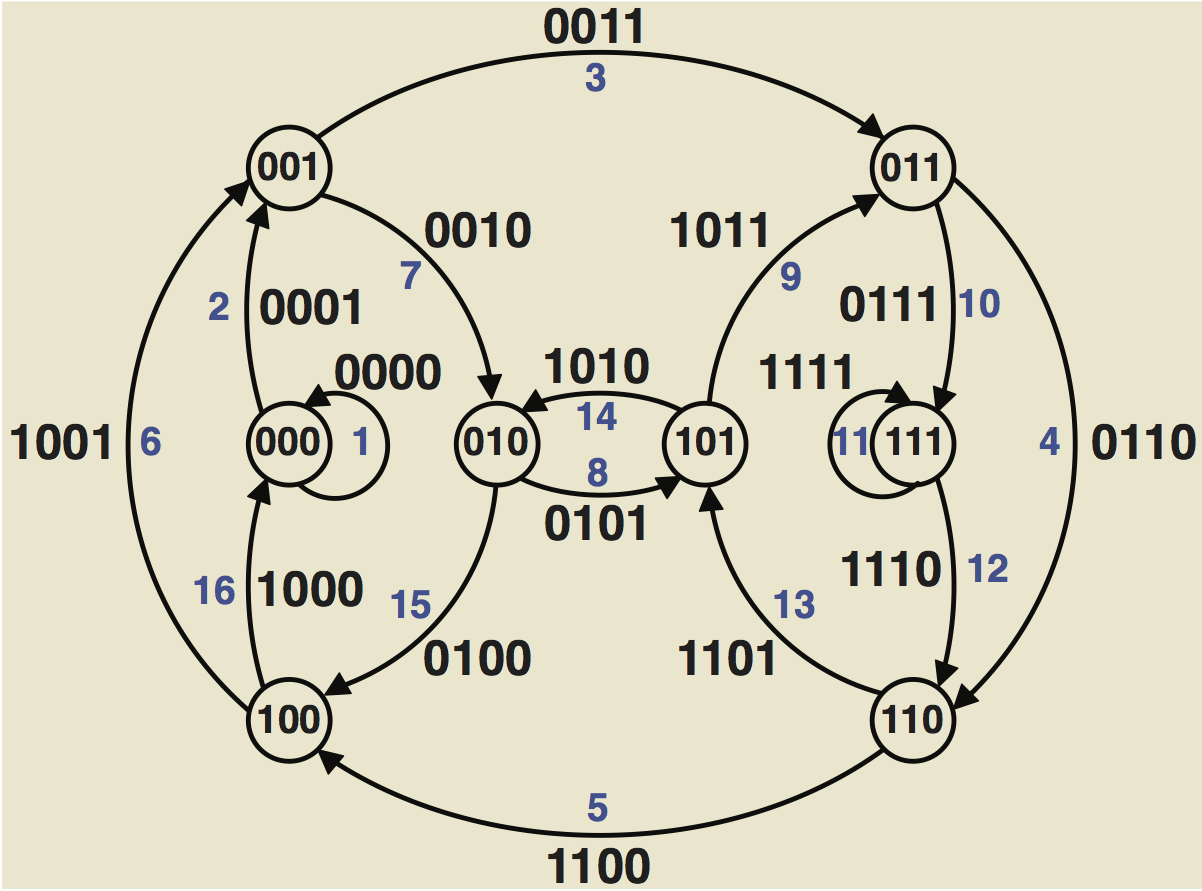
\includegraphics[scale=0.4]{debruijn.png}
  \end{center}
  \caption{deBruijn çizgesi.}
  \label{fig:debruijn}
\end{figure}

de Bruijn çizgelerinin en önemli özelliği Euler döngüsü içeriyor olmalarıdır. Bunun sebebi çok basittir: her köşeye $n$ tane giren kenar ve her köşeden $n$ tane çıkan kenar vardır. Ayrıca, bu çizgenin üzerindeki Euler döngüsü çizgedeki bütün kenarları içerdiği için, bu Euler döngüsü sayesinde ortaya çıkan dizi de $k$ uzunluğundaki olabilecek bütün nk farklı diziyi de içermektedir. Dolayısıyla, Euler döngüsü en baştaki probleme çözüm üretmiş olur.

	Bu noktada karşılaştığımız soru, yukarıda anlatılan de Bruijn çizgesini genom birleştirme problemine nasıl uygulayabileceğimiz olacaktır. Gözlemlenmesi gereken ilk nokta genom birleştirme problemindeki alfabenin 4 harften oluşmasıdır: $\{A, T, G, C\}$. $k$ sayısı ise 50 ve 75 aralığında sabit bir sayı olarak seçilir (100 baz çiftlik diziler için). Seçilen $k$ sayısı kullanılarak her kısa dizinin $k-1$ uzunluğundaki bütün altdizileri ($(k-1)$-mers) bir araya getirilir. Bu $(k-1)$-mer'ler, oluşturulan de Bruijn çizgesindeki köşelere denk gelmektedirler. Kısa dizilerde art-arda gelen ve $k-2$ harfi örtüşen herhangi iki $(k-1)$-mer için de Bruijn çizgesine birer kenar eklenir. Bu eklenen kenar ait olduğu iki $(k-1)$-mer'den oluşan $k$ uzunluğundaki diziye tekabül etmektedir.
	Kısa dizilerinin çok fazla sayıda olması ve $k$ sayısının küçük olması, oluşturulan de Bruijn çizgesinin olası tüm $4^k-1$ tane köşeyi ve $n^k$ tane kenarı içerdiğini varsayabiliriz. Dolayısıyla, oluşturulan de Bruijn çizgesi Euler döngüsü içermektedir ve bu döngünün oluşturduğu uzun dizi tüm kısa dizileri içerdiği için bizim aradığımız hedef genom dizisine denk gelir.
	Elimizdeki milyarlarca kısa diziden oluşturulan de Bruijn çizgesi genomdaki dizi tekrarlanması problemini çözemez. Bunun en başlıca sebebi kısa dizilerin hedef genomu eşit dağılmadan kapsamasıdır. Dolayısıyla, oluşturulan çizgenin kenar ağırlıklarının yüksek olduğu kısımlar aslında birden fazla tekrarlana diziye mi yoksa tekrarlanmayan ama dizileme sırasında çok fazla kapsanan diziye mi tekabül ettiğini ayırt etmek zor bir problemdir. Şekil~\ref{fig:debruijn-repeat} tekrarlanan dizilerin çizge üzerindeki etkilerini göstermektedir:

\begin{figure}[htb]
  \begin{center}
    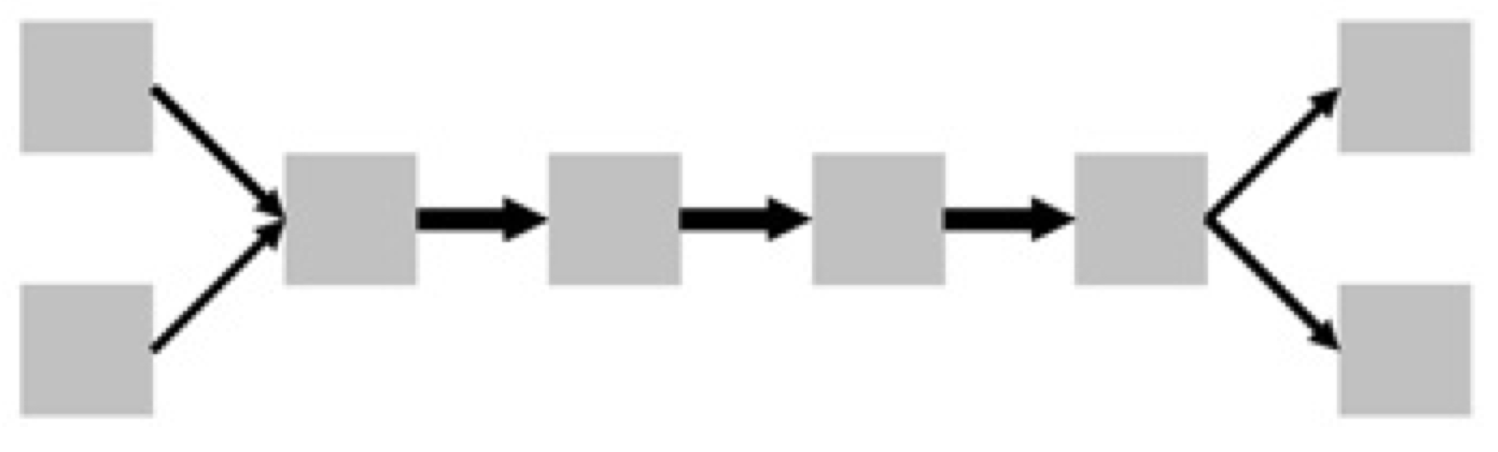
\includegraphics[scale=0.4]{debruijn-repeat-problem.png}
  \end{center}
  \caption{Tekrarlanan dizilerin deBruijn çizgesi üzerindeki etkileri.}
  \label{fig:debruijn-repeat}
\end{figure}

	Şekil~\ref{fig:debruijn-repeat}'de görüldüğü gibi kısa dizilerin uzunluklar tekrarlanan dizilerin uzunluklarından daha kısa (şekildeki köşeler kısa dizilere denk gelmektedir) olduğunda bu tür sorunlar oluşuyor. Ortadaki kalın kenarlar Euler döngüsünde 2 farklı yerde kullanılması gerekirken tek yerde kullanılacaktır. Bu sorunu çözmek için dizileme hata payı yüksek olmasına rağmen ürettiği kısa dizilerin uzunlukları çok uzun olan bir başka dizileme teknolojisinin ürettiği verileri de kullanarak hiperçizge (hypergraph) yapısı altında  yeni bir genom birleştirme algoritması öneriyoruz. Önerdiğimiz yöntemin detaylarına inmeden önce hiperçizge yapısını tanımlayalım:
	
	Hiperçizge $H = (V, X)$ çiftinden oluşmaktadır. $V$ köşelerin kümesini tanımlar, $X = \{E_1, E_2, \ldots, E_n\}$ ise hiperkenarları tanımlar. Burada, $X$ kümesi $V$'nin altkümelerinden oluşur ve $|E_i| \geq 2$ kuralını sağlar. Genel olarak, hiperçizgelerin normal çizgelerden en önemli farkı, hiperkenarların sadece iki köşeyi değil, ikiden fazla köşeyi de birleştirebiliyor olmasıdır.

	Günümüz Yeni Nesil Dizileme cihazlarından iki tanesini ele alalım:

\begin{itemize}
\item Illumina: Dizileme sonucunda ürettiği kısa dizilerin uzunluğu 100-150 baz çiftidir. Uzunluk çok kısa olmasına rağmen, bu teknolojinin hata payı 0.01\% civarındadır.
\item Pacific Biosciences (PacBio): Dizileme sonucunda ürettiği kısa dizilerin ortalama uzunluğu 8000 baz çifti civarındadır. Ancak diziler uzun olmalarına rağmen, bu teknolojinin hata payı 10\%-15\% civarındadır.
\end{itemize}

	Illumina'nın çıktılarının hata payı çok düşük olduğu için, bu teknoloji çok yaygın kullanılmaktadır. Ancak kısa dizilerin uzunluğu 100 baz çifti olduğu için, hedef genomdaki uzunluğu 100'den daha uzun olan tekrarlanan dizilerin belirlenmesi çok zordur. Bizim önerdiğimiz çözüm 2 aşamalıdır:

\begin{enumerate}
\item Geleneksel de Bruijn çizgesi yöntemini ve sadece Illuminadan gelen verileri kullanarak de Bruijn çizgesinin oluşturulması.
\item PacBio cihazından gelen her bir kısa dizi için 1. aşamada oluşturulan çizgeye 1 tane hiperkenarın eklenmesi. Bu eklenen hiperkenar, ait olduğu kısa dizinin içerdiği tüm $(k-1)$-merleri birleştirir. 
\end{enumerate}

İki aşama sonucunda elde edilen hiperçizge Şekil~\ref{fig:hypergraph}'de gösterilmiştir.

\begin{figure}[htb]
  \begin{center}
    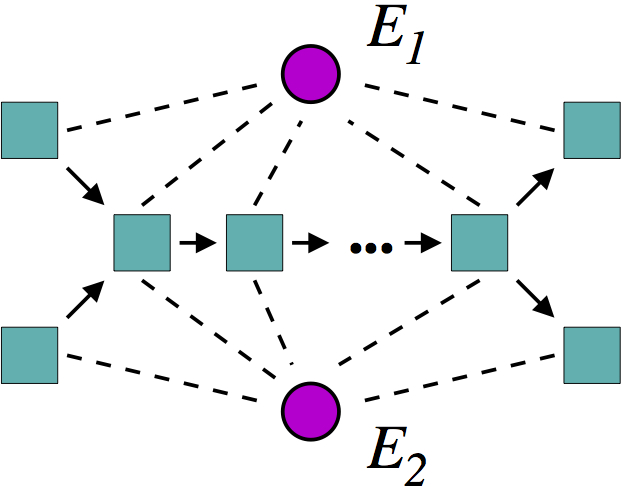
\includegraphics[scale=0.4]{hypergraph.png}
  \end{center}
  \caption{Hiperçizge.}
  \label{fig:hypergraph}
\end{figure}



	Bu modellemenin avantajları aşağıda listelenmiştir:
PacBio'dan gelen kısa dizilerin uzunlukları kadar uzun tekrarlanmalar çözümlenebilir.
PacBio'nun dizileme hata payı çok yüksek olmasına rağmen, elde edilen nihai genom Illumina verisinden elde edilen verinin hata payına göre oluşturulur.
Bu model sadece bu iki veri kaynağı için değil, başka veri kaynaklarından gelen veriler için de kullanılabilir; örneğin Roche/454, Ion Torrent, Oxford Nanosciences, Moleculo, vb.



\clearpage

{\bf \large 3.5. Ekzom Dizilemede GC ve Yakalama Verimi Hatalarının Düzeltilmesi}
\addcontentsline{toc}{subsection}{3.5. Ekzom Dizilemede GC ve Yakalama Verimi Hatalarının Düzeltilmesi}

DNA'nın sadece belirli bölgelerinde yaşanan dizi değişimlerine bakmak için tüm genom birleştirme yöntemini kullanmak yerine hedefleyici birleştirme yöntemini kullanmak daha etkin sonuçlar vermektedir. Hedefleyici birleştirme yönteminin alt sınıflarından birisi de yalnızca protein kodlayan bölgeleri hedefleyen ekzom birleştirme yöntemidir. Ancak ekzom birleştirme metodunu kullanabilmek için ekzon verilerindeki GC-içeriği ve ekzon yakalama etkinliği gibi bazı sapmaları düzeltmek gerekmektedir (Şekil~\ref{fig:exomedepth}). Bu sapmalardan GC-içeriğini düzeltmek için yapılmış birçok çalışma olmasına rağmen~\cite{Krumm2012,Fromer2012} ekzon yakalama etkinliğiyle alakalı bilinen bir çalışma bulunmamaktadır. Bu alandaki açığı kapatarak ekzom birleştirme yöntemini de kullanabilmek için bir çalışma yaptık. Prob yakalama etkinliğinde varolan sapmaları düzeltmek için yaptığımız bu çalışma sonucunda bu etkiyi büyük ölçüde düzelttik. 


\begin{figure}[htb]
\begin{center}
  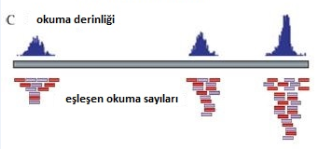
\includegraphics[scale=0.75]{exomedepth.png}
\end{center}
\caption{Okumaların 3 farklı ekzom bölgesine eşleştirilmesi. Her üç ekzonun da kopya sayısı aynı olmasına rağmen GC profili ve yakalama etkinliğindeki farklılıklar nedeniyle dizileme derinlikleri farklı görünebilmektedir.}
\label{fig:exomedepth}
\end{figure}

 Prob yakalama etkinliği, genomun her yerinde o bölgede kullanılan probun özelliklerine göre değişmektedir. Her bölgenin bu sapmadan ne kadar etkilendiğini görmek ve bu sapmaları düzeltebilmek için, dizileme teknolojileri kullanılarak elde edilen DNA parçacıklarını ekzon koordinatlarına göre eşleştirdik. Daha sonra her bir bölgeye ait prob sayısı ve dizi derinliğine bakılarak, yakalama etkinliklerini tespit ettik. 

{\bf 3.5.1. Birden Fazla Örnek Üzerinde Çalışabilmek için Ekzom Dizileme Verilerinin Uyarlanması}
\addcontentsline{toc}{subsubsection}{3.5.1. Birden Fazla Örnek Üzerinde Çalışabilmek için Ekzom Dizileme Verilerinin Uyarlanması}

Ekzom dizilemesi verilerinin üzerinde çalışırken, örneklere ait verilerin okuma derinlikleriyle kopya sayısı varyantlarını kıyaslayabilmek için pencere büyüklüklerini (window size) eşitlememiz gerekmektedir. Bunu yapabilmek için her bir ekzona map edilmiş olan okuma sayısının ortalaması (exome mean read count)(EMRC) hesaplanmalıdır. EMRC aşağıdaki gibi formülize edilmiştir:

\[ERMC_e = \frac{RC_e}{L_e}\]

Burada $RC_E$ hedeflenen e genomik bölgesine eşleştirilen okuma sayısını, $L_e$ ise aynı genomik bölgenin büyüklüğünü ifade etmektedir. EMRC genomun edeflenen her bir bölgesi için hesaplanıp, belirli bölgelere eşleştirilen okuma yoğunluğunun bir ölçüsünü vermektedir. 

{\bf 3.5.2. GC İçeriği Yanlılığı}
\addcontentsline{toc}{subsubsection}{3.5.2. GC İçeriği Yanlılığı}

GC içeriği yanlılığı, okuma kapsamı (read coverage) ile dizileme verisinde bulunan GC içeriğinin arasındaki ilişkiyi ifade etmektedir. Bu yanlılık, DNA dizilemesinde varolan kopya sayısı tahmininde de olabileceği gibi, genomdaki parça (fragment) bolluğunu ölçmeye odaklı analizlerdeki sinyalleri domine edebilmektedir. Ayrıca örnekler arasında tutarlılık gösteren bir yanlılık olmayıp, tek bir örnekteki yanlılığı ortadan kaldırabilecek en iyi yöntem diye bir şeyden de söz edilememektedir.

{\bf 3.5.3. Batch Etkisi}
\addcontentsline{toc}{subsubsection}{3.5.3. Batch Etkisi}

Genetik varyantlar, gen ve protein ifadelerinde ve epigenetik modifikasyonlar için geniş ölçekte kullanılan  YND teknolojileri, gözden kaçırılabilecek batch etkisine sık sık maruz kalabilmektedir. Batch yanlılığı laboratuvar şartlarından ve personel değişimleri gibi durumlardan meydana gelebilmektedir. Bu etki,  verdiği doğru olmayan sonuçlara bağlı olarak çok önemli bir problem haline gelmiştir.


{\bf 3.5.4. Temel İçerik Analizi (Principal Component Analysis)(PCA)}
\addcontentsline{toc}{subsubsection}{3.5.4. Temel İçerik Analizi (Principal Component Analysis)(PCA)}

Temel içerik analizi, modern veri analizinin dayanak  noktası haline gelmiştir. Bunun yanı sıra uygulamalı lineer cebirin en değerli sonucu olarak da kabul edilmektedir. PCA olarak da bilinen bu yöntem çok yaygın bir şekilde ancak çok iyi anlaşılmadan kullanılmaktadır. Bu da yanlış sonuçlar doğurmaktadır. Yürütmekte olduğumuz çalışmada PCA yönteminin olası yanlış kullanımlarını düzelterek, daha doğru veriler de elde etmeyi hedeflemekteyiz. Karmakarışık bir veri kümesinden, en alakalı kısmı alabilen parametrik olmayan bir metot olduğu için nöroloji biliminden bilgisayar grafiği alanına kadar geniş bir yelpazede kullanılmaktadır. Minimal düzeyde ek bir çaba ile PCA, kompleks bir veri kümesinden kümeyi ifade edebilen küçük bir data setini elde edebilmeyi, zaman zaman ise gizli kalmış altta yatan basit dinamiklerin ortaya çıkarılmasını sağlamaktadır. PCA'nın amacı,  pürüzlü (noisy) veri kümesini en anlamlı ve daha basit bir şekilde yeniden ifade edebilmeyi sağlamaktır.

\clearpage
{\bf 3.5.5. Değişken Bayes Çıkarımı}
\addcontentsline{toc}{subsubsection}{3.5.5. Değişken Bayes Çıkarımı}


Tekil değer ayrışımı (SVD), bir matrisin optimal bir şekilde düşük rank ayrımını (karesel hata anlamında), döndüren bir matris  ayrıştırma algoritmasıdır. SVD'nin; çıktısı, verinin kompakt ve bilgilendirici bir gösterimi olarak yorumlanabilecek makine öğrenimi uygulamalarında geniş bir kullanımı vardır. Maalesef bunun yanında, aşırı aralıklı matrisler için veriye gereğinden fazla uyumlu grafikler ortaya çıkararak, yeni verinin grafikte doğru bir şekilde yer bulmasını engelleyebilmektedir. Bu nedenle çok dikkatli bir şekilde ele alınmalıdır. Kopya sayısı varyantı tespiti algoritmalarında da  oldukça fazla kullanılmaktadır.

Elimizde var olan (kopya sayısı) $\times$ (örnekler) matrisinin  ekzom datasına bağlı olarak gelişen aralıklı yapısından dolayı SVD bazen yeterli olamamaktadır. Burada oluşabilecek verinin fazla uyumlu grafikler ortaya çıkarabilmesi durumunu engelleyebilmek için her biri veri kümesinin yapısına uygun parametreler ve yapılar ortaya çıkaran değişken bayes çıkarımını kullanmayı planlamaktayız. Elimizdeki veri kümesine oldukça benzeyen daha önce internet sitelerinde yer alan sinema tavsiyeleri için makine öğrenmesi uygulamasında da kullanılmış ve buradaki sonuçları iyileştirmiştir.

{\bf 3.5.6. GC ve yakalama etkinliğinden doğan farklılıkların düzeltilmesi}
\addcontentsline{toc}{subsubsection}{3.5.6. GC ve yakalama etkinliğinden doğan farklılıkların düzeltilmesi}

Elimizdeki veriyi matris benzeri bir yapı olarak düşünebiliriz. Bunlardan ilki; (okuma derinliği) $\times$ (örnek), ikincisi; (kopya sayısı varyantı) $\times$ (örnekler) matrisidir  diyebiliriz. Okuma derinliği verisini içeren ilk matrisimizde eksik veri bulunmamaktadır. Amacımız ilk matristeki verileri kullanarak, fazla sayıda eksik veri içeren ikinci matrisimizdeki kopya sayısı varyantlarını tespit edebilmektir. Elimizde varolan veriler tüm genom dizilemesi verileridir. Biz bu verileri daha önceden elde edilmiş insan ekzom verisiyle eşleştirdik(mapping). Böylece kopya sayısı varyantı tespitinde daha avantajlı DNA'nın sadece ekzom kısmıyla ilgilenebiliyoruz. Eşleştirdikten sonra matrislerin üzerinde işlem yapabilmemiz için farklı örneklerden  geliyor olmasından kaynaklanan pencere büyüklüğü sorununu çözebilmek için daha önce bahsetmiş olduğumuz ``Birden Fazla Örnek Üzerinde Çalışabilmek için Ekzom Dizileme Verilerinin Uyarlanması'' kısmındaki EMRC formülünü kullanarak uniform matrisler elde etmekteyiz.

Bilindiği üzere kromozomlar eşey ve otozomal kromozomlar olarak iki grupta toplanmaktadır. Bu iki tür kromozom farklı yapılarından dolayı ayrı ayrı ele alınmalıdır. Bu sebeple ilk aşamada otozomal kromozomlar üzerinde çalışacağımız için ekzon dizilemesinden eşey kromozomları olan X ve Y kromozomlarına dair veriler çıkarıldı. 

Elimizde bulunan kopya sayısı varyantı verilerinde 2, normal kopya sayısı; 0-1 delesyon; 3 ve daha fazlası duplikasyon görüldüğünü belirtmektedir. 1000 Genom Projesi'nden~\cite{1000GP2012} mevcut populasyonlara ait örneklemlerin (sample) deletion kısımları alındı. Daha sonra bu deletionların arasından bütün örneklemlerde ortak olarak görülen deletionlar alındı. Alınan bu deletionlar ile daha önceden elde etmiş olduğumuz verilerin kesişmeyen kısımları ``normal'' yani 2 olarak kabul edildi.

Bu veri kümesinde GC ve yakalama prob sayıları ile dizileme derinliği arasındaki ilişkiyi anlayabilmek için ykarıda anlatıldığı üzere kopya sayısı varyasyonu bulunmayan bölgelerde korelasyon hesaplaması yaptık. Bu bölgelerde varyasyon bulunmadığı için normal dağılımda tüm ekzonların dizileme derinliğinin aynı olması beklenir, ancak GC değerleri ve yakalama prob sayılarının farklılıkları nedeniyle farklı derinlikler gözlenmektedir (Şekil \ref{fig:exomedepth}). Korelasyon katsayılarını aşağıdaki şekilde hesapladık:

\[r_{rd,pr} = \frac{\sum_{i=1}^{n}(rd_i-\overline{rd})(pr_i-\overline{pr})}{\sqrt{\sum_{i=1}^{n}(rd_i-\overline{rd})^2\sum_{i=1}^{n}}(pr_i-\overline{pr})^2} \]
\[r_{rd,gc} = \frac{\sum_{i=1}^{n}(rd_i-\overline{rd})(gc_i-\overline{gc})}{\sqrt{\sum_{i=1}^{n}(rd_i-\overline{rd})^2\sum_{i=1}^{n}}(gc_i-\overline{gc})^2} \]

\paragraph{Çoklu korelasyon.}
Çoklu korelasyon bir bağımlı değişkenin çok sayıda bağımsız değişken ile arasındaki lineer bağlamı ölçer. Bu şekilde modelde birden fazla değişkenin kullanılıp kullanılmayacağına karar vermek için kullanılır. GC içerigi (gc) ve prob sayısını (pr) bağımsız, dizileme derinliğini (rd) bağımlı değişken olarak alıp çoklu korelasyon katsayısını aşağıdaki şekilde hesapladık:

\[R_{rd,pr,gc} = \frac{\sqrt{r_{rd,gc}^2 + r_{rd,pr}^2 - 2r_{rd,gc}r_{rd,pr}r_{gc_pr}}}{\sqrt{1-r_{gc,pr}^2}}\]

Burada $r_{rd,gc}$ derilik ve GC arasında, $r_{rd,pr}$ derinlik ve prob sayısı arasında, $r_{gc,pr}$ de GC ve prob sayısı arasındaki ikili korelasyonu ifade eder.
\vspace*{-0.2cm}
\paragraph{Veri düzleştirme (LOESS).} 
LOESS metodu yerel ağırlıklı lineer gerileme kullanarak verilerin düzleştirilmesini sağlar. Düzlük katsayısı dışında bir parametreye ihtiyaç duymaz. Verinin aşağıdaki gibi bir fonksiyon ile üretildiği varsayılır:
\[y_i = g(x_i) + \epsilon_i\]
Burada $g$, bağımsız değişkenler arasındaki düzlük katsayısını ifade eden bir fonksiyondur.

%LOESS metodu ile veri düzeltme işlemi aşağıdaki gibidir:

%$x_i$'nin $n$ farklı değişken ve $y_i$'in hesaplanan değer olduğu durumda:

%\begin{enumerate}
%\item
%  0 ve 1 arasında bir düzlük katsayısı seçilir (\alpha) Daha sonra $k$ değeri $\alpha\times n$ %değerine eşit ya da daha az olacan şekildeki en büyük tamsayı olarak hesaplanır.
%\item
%  Veri kümesindeki her $x_0$ için en yakın $k$ nokta bulunur. 
%\item
%\item
%\item
%\item
%\item
%\end{enumerate}

\clearpage
\begin{center}
{\bf \Large 4. BULGULAR}
\end{center}
\addcontentsline{toc}{section}{4. BULGULAR}
\noindent

{\bf \large 4.1. Havuzlanmış klon dizileme ile genom iskeleleme}
\addcontentsline{toc}{subsection}{4.1. Havuzlanmış klon dizileme ile genom iskeleleme}

Bu projede kullandığımız programları hem en uzun (kromozom 1), hem de en kısa (kromozom 20) verileri üzerinde test ettik. Her iki kromozom için ikişer farklı strateji uyguladık. Önce havuzlanmış BYK verilerinin tümünü kullanarak iskeleleme yaptık (Tablo~\ref{tab:chr1w}, \ref{tab:chr20w}), 
daha sonra havuzları sırayla teker teker ekleyerek iskeleleme deneyi 
yaptık (Tablo~\ref{tab:chr1h}, \ref{tab:chr20h}). Sonuç olarak
tüm genom verileri için geliştirilen iskeleleme algoritmalarının, BYK ve fosmid verisi kullanıldığında genom birleştirme kalitesine bir fayda sağlamadığını gözlemledik.

\begin{table}[htb]
\caption{Kromozom 1 verileri üzerinde tüm BYK verilerini birleştirerek yaptığımız iskeleleme sonuçları.}
\label{tab:chr1w}
\begin{center}
\begin{tabular}{|l|r|r|r|r|r|r|r|}
\hline 
{\bf Algoritma } & {\bf İskele} & {\bf Toplam bp} & {\bf ATCG} & {\bf GC\%} & {\bf N} & {\bf N50} & {\bf N90} \\
\hline
SSPACE & 9,891 & 121,405,472 & 121,404,200 & 41.57 & 1,272 & 28,279 & 5,757\\
SCARPA &  \textit{NA}  &  \textit{NA}     &     \textit{NA}  &   \textit{NA}   &  \textit{NA}    &  \textit{NA}    &  \textit{NA}   \\
OPERA  & 9,408     & 121,412,030      & 121,400,964     & 41.57  &  11,066   & 28,159    & 5,757   \\
BESST  & 7,028	& 99,697,046	& 99,595,402	& 42.12 &	101,644 &	32,938 &	6,708 \\ 
\hline
\end{tabular}
\end{center}
\end{table}


\begin{table}[htb]
\caption{Kromozom 20 verileri üzerinde tüm BYK verilerini birleştirerek yaptığımız iskeleleme sonuçları.}
\label{tab:chr20w}
\begin{center}
\begin{tabular}{|l|r|r|r|r|r|r|r|}
\hline 
{\bf Algoritma } & {\bf İskele} & {\bf Toplam bp} & {\bf ATCG} & {\bf GC\%} & {\bf N} & {\bf N50} & {\bf N90} \\
\hline
SSPACE & 249	& 10,019,741	& 10,019,735	&  44.75	& 6	& 49,769	& 22,871 \\
SCARPA & 248	& 10,019,787	& 10,019,735	& 44.75	& 52	& 50,183	& 22,871  \\
OPERA  & 248	& 10,019,760	& 10,019,686	& 44.75	& 74	& 50,183	& 23,331 \\
BESST  & 115	& 4,683,891	& 4,683,167	& 45.44	& 724	 & 48,117  	& 23,589 \\
\hline
\end{tabular}
\end{center}
\end{table}


\begin{table}[htb]
\caption{Kromozom 1 verileri üzerinde BYK havuzlarını sırayla birleştirerek yaptığımız iskeleleme sonuçları.}
\label{tab:chr1h}
\begin{center}
\begin{tabular}{|l|r|r|r|r|r|r|r|}
\hline 
{\bf Algoritma } & {\bf İskele} & {\bf Toplam bp} & {\bf ATCG} & {\bf GC\%} & {\bf N} & {\bf N50} & {\bf N90} \\
\hline
SSPACE & 9,569       & 121,501,965        & 121,491,831 & 41.57 & 10,134 & 29,121 & 5,936 \\
SCARPA &  \textit{NA}  &  \textit{NA}     &     \textit{NA}  &   \textit{NA}   &  \textit{NA}    &  \textit{NA}    &  \textit{NA}   \\
OPERA  & 9,897       & 121,406,580        & 121,403,836 & 41.57 & 2,744  & 28,531 & 5757 \\
BESST  & 513 & 1,564,335          & 1,564,334   & 50.66 & 1     & 4,520  & 1,319 \\ 
\hline
\end{tabular}
\end{center}
\end{table}


\begin{table}[htb]
\caption{Kromozom 20 verileri üzerinde BYK havuzlarını sırayla birleştirerek yaptığımız iskeleleme sonuçları.}
\label{tab:chr20h}
\begin{center}
\begin{tabular}{|l|r|r|r|r|r|r|r|}
\hline 
{\bf Algoritma } & {\bf İskele} & {\bf Toplam bp} & {\bf ATCG} & {\bf GC\%} & {\bf N} & {\bf N50} & {\bf N90} \\
\hline
SSPACE &  \textit{NA}  &  \textit{NA}     &     \textit{NA}  &   \textit{NA}   &  \textit{NA}    &  \textit{NA}    &  \textit{NA}   \\
SCARPA &   247	& 10,019,775 &	10,019,735	& 44.75	& 40	& 5,018 &	23,331\\
OPERA  &  250	& 10,019,740	& 10,019,735	& 44.75	& 5	& 49,272	& 22,521 \\
BESST  &  17    & 308,948 & 308,948  & 47.81 & 0  & 22,521 & 10,538 \\ \hline
\end{tabular}
\end{center}
\end{table}

%\clearpage

{\bf \large 4.2. Birden fazla platform verisi ile genom birleştirmelerde hata düzeltimi}
\addcontentsline{toc}{subsection}{4.2. Birden fazla platform verisi ile genom birleştirmelerde hata düzeltimi}


Sonuçların özeti Tablo \ref{tab:resultsTable}'de sunulmuştur. 
Özetlersek, sadece Illumina okumalarıyla Velvet kullanılarak yapılan birleştirme uzun okumalarla Celera kullanılarak yapılan birleştirmeye göre daha yüksek kapsama (\%99) ve ortalama benzerlik (\%97.5) gösterdi.

Celera birleştirmesini bizim metodumuzla düzeltmek hem kapsama hem de ortalama benzerlik oranlarını artırıyor, daha sonra da sonuç tekrarlı doğrulamalar ile daha da iyileştiriliyor.
İlk doğrulama tekrarında 454-Celera birleştirmesinin kapsaması \%99.7'ye kadar ortalama benzerliği de \%94.4'e kadar yükseliyor. 
Tekrarlı doğrulama döngüleri kapsama ve ortalama benzerlik oranlarını artırıyor. 
Döngüler eğer ortalama benzerlik değerinde bir yükselme yoksa veya kapsama oranının artmasından dolayı bir düşüş yaşanıyorsa son buluyor. 

Tüm birleştiricilerin sonuçları için uzun okumalardan elde edilen birleştirmelerin kısa okumalardan elde edilen birleştirmelerle düzeltilmesinin iyi çalıştığını görebilirsiniz. 
Yalnız, düzeltilmiş SGA birleştirmesi içlerinde en iyi kapsama oranına sahip.
Ayrıca, kısa ve uzun okumaları ayrı ayrı de Bruijn ve OLC çizge tabanlı birleştiricilerle birleştirmek ve sonrasında onları birbirleriyle düzeltmek, tüm okumaları birlikte tek seferde Masurca veya Celera-CABOG gibi bir hibrid birleştirici ile birleştirmekten daha iyi sonuç veriyor. Masurca en iyi ortalama benzerliğe Illumina-Ion-Torrent verisinde sahip gibi görünüyor fakat kapsama oranı sadece \%1. 
Celera-CABOG aslında Illumina-454 verisi üzerinde gayet iyi çalışıyor, ama Illumina ve 454 okumaları kullanarak doğrulanmış SGA veya doğrulanmış Celera kadar iyi değil. 
Celera-CAGOB Illumina-Ion-Torrent verisi ile çalıştırıldığında referans ile eşleşen hiç bitişik elde edilemiyor, tüm bitişikler kontaminasyon eleme aşamasında eleniyor.

Sonuç olarak farklı NGS teknolojilerinden elde edilen değişik veri türlerinin özelliklerinden (uzun/kısa okumalar, yüksek/düşük kaliteli okumalar) yararlanmak için yeni metodların geliştirilmesi ihtiyacı devam ediyor. 
Bu bakımdan gelecek iş olarak, doğrulama algoritmamızı kısa eşli okumalardan yararlanarak doğrulama aşamasından sonra doğrulanmış bitişiklerin arasındaki boşlukları doldurmak için kullanıp birleştirmeyi daha da iyileştirebiliriz.
 

\begin{table}[htb]
\begin{center}
{\footnotesize
\begin{tabular}{l|l|l|l|l|l|l|l|l|}
\hline
         İsim & Uzunluk & \# (Bitişik) & \thead{\# (Eşleşen \\ bitişik)} & \thead{\# (Kaps.\\ baz)} & Kapsam & \thead{Ort. \\özdeşlik} & \# (Boşluk) & \thead{Boşluk \\ boyutu} \\
\hline
	 \textbf{\textit{Referans}} & \textit{176.843} & & & & & & & \\
\hline	 
	 \textbf{Velvet} & & & & & & & & \\
         Ill. Velvet & 197,040 & 455 & 437 & 175,172 & 0.99055 & 0.97523 & 39 & 1,671 \\
         \textbf{Celera} & & & & & & & & \\       
         454 Celera & 908,008 & 735 & 735 & 172,563 & 0.97580 & 0.92599 & 18 & 4,280 \\
         Ion Celera & 39,347 & 27 & 27 & 47,638 & 0.26938 & 0.96932 & 47 & 129,205 \\
         \hline   
         \textbf{Corrected Celera} & & & & & & & & \\
         Ill-454 Celera & 4,945,785 & 895 & 270 & 176,368 & 0.99731 & 0.94370 & 5 & 475 \\
         Ill-454 Celera$^{2*}$ & 5,078,059 & 890 & 265 & 176,640 & 0.998852 & 0.944527 & 4 & 203 \\
         Ill-Ion Celera & 93,909 & 30 & 28 & 81,819 & 0.46267 & 0.96327 & 36 & 95,024 \\
         Ill-Ion Celera$^2$ & 145,262 & 30 & 28 & 91,962 & 0.52002 & 0.97412 & 33 & 84,881 \\
         Ill-Ion Celera$^3$ & 216,167 & 30 & 28 & 99,645 & 0.56347 & 0.98066 & 34 & 77,198 \\
         \textbf{SGA} & & & & & & & & \\
         454 SGA & 62,909,254 & 108,095 & 101,514 & 176,546 & 0.99832 & 0.97439 & 1 & 297 \\
         Ion SGA & 842,997 & 6,417 & 6,122 & 153,092 & 0.86569 & 0.99124 & 197 & 23.751 \\	
         \hline
         \textbf{Corrected SGA} & & & & & & & & \\
         Ill-454 SGA & 295,009 & 335 & 335 & 176,757 & 0.99951 & 0.96823 & 5 & 86 \\
         Ill-454 SGA$^2$ & 279,034 & 305 & 305 & 176,757 & 0.99951 & 0.96769 & 5 & 86 \\
         Ill-Ion SGA & 197,509 & 291 & 291 & 175,052 & 0.98987 & 0.97501 & 45 & 1,791 \\
         Ill-Ion SGA$^2$ & 203,064 & 291 & 291 & 175,676 & 0.99340 & 0.97413 & 34 & 1,167 \\
         \textbf{SPADES} & & & & & & & & \\
         454 SPADES & 12,307,761 & 49,824 & 49,691 & 176,843 & 1.0 & 0.98053 & 0 & 0 \\
         Ion SPADES & 176,561 & 110 & 107 & 167,890 & 0.94937 & 0.92909 & 9 & 8,953 \\	
         \hline
         \textbf{Corrected SPADES} & & & & & & & & \\
         Ill-454 SPADES & 290,702 & 298 & 298 & 176,454 & 0.99780 & 0.96538 & 5 & 389 \\
         Ill-Ion SPADES & 198,665 & 52 & 52 & 171,977 & 0.97248 & 0.94215 & 4 & 4,866 \\
         Ill-Ion SPADES$^2$ & 200,307 & 52 & 52 & 172,101 & 0.97319 & 0.94230 & 2 & 4,742 \\
         \textbf{Masurca} & & & & & & & & \\
         Ill-454 Masurca & 380 & 1 & 0 & 0 & 0 & 0 & 0 & 0 \\
         Ill-Ion Masurca & 2,640 & 8 & 8 & 1,952 & 0.01104 & 0.98223 & 9 & 174,891 \\
 		\textbf{Celera-CABOG} & & & & & & & & \\
         Ill-454 Celera & 1,101,716 & 891 & 891 & 174,330 & 0.98579 & 0.92452 & 12 & 2,513 \\
         Ill-Ion Celera & 0 & 0 & 0 & 0 & 0.0 & 0.0 & 0 & 0.0 \\
\hline
\end{tabular}
}
\end{center}
{\footnotesize İsim: Birleştirmeyi oluşturan veri grubunun adı; Uzunluk: Toplam birleştirme uzunluğu \#(Bitişik): Sonuçta elde edilen birleşmeye ait bitişik sayısı; \#(Eşleşen bitişik): Başarılı bir şekilde referansa eşleşen bitişik sayısı; \#(Kaps. baz):  Birleştirme tarafından referans üzerinde kapsanan baz sayısı; Kapsam: Kapsanan referans yüzdesi; Ort. özdeşlik: Doğru bir şekilde tahmin edilmiş referans baz sayısı; \#(Boşluk): Referans genom üzerinde kapsanamamış boşluk sayısı; Boşluk boyutu: Boşluklar üzerindeki toplam baz sayısı.
  ``2'' ikinci doğrulama devrini temsil ediyor, ``3'' üçüncü devri temsil ediyor.}
\caption{BAC verisi üzerinde birleştirme doğrulama yöntemine ait sonuçlar.}
\label{tab:resultsTable}

\end{table}






%\clearpage

{\bf \large 4.3. Illumina ve PacBio verilerini kullanan hibrit birleştirme algoritması}
\addcontentsline{toc}{subsection}{4.3. Illumina ve PacBio verilerini kullanan hibrit birleştirme algoritması}

{\bf 4.3.1. Hızlı Illumina-PacBio hizalanması için filtreleme}
\addcontentsline{toc}{subsubsection}{4.3.1. Hızlı Illumina-PacBio hizalanması için filtreleme}

İkinci filtre uygulanmadan önce hangi parametrelerin seçilmesi gerektiğini yorumlamak adına öncelikle ilk filtrede elde edilen sonuçları sunacağız. Parametreleri belirlerken doğru yapılan eleme oranıyla yanlış yapılan eleme oranı arasında bir denge belirlemekteyiz. Her iki filtreyi uygularken de elenmemesi gereken eşlerin mümkün olduğunca en az sayıda eleniyor olduğunu kontrol ediyor olacağız. Bu sebeple, ilk filtre elenmesi gerekenlerin büyük çoğunu elemiyor olsa bile, eğer \%90 veya daha fazla oranda elenmemesi gereken eşler de bu filtreden geçebiliyorsa bizim için hala ilk filtrede kullanılan paramatreler uygulanabilir olacaktır. İkinci filtre daha hassas bir eleme yapacağından dolayı, SW metodunda hizalanmayacak olan eşlerin, ikinci filtreyi de geçemeyeceği varsayımı öngörülebilir bir varsayımdır. Çeşitli parametrelerin seçimiyle oluşan sonuçlar tablolarda verilmiştir. Sayfa \pageref{table:results1} Tablo \ref{table:results1} ne kadar doğru ve yanlış elemelerin birinci filtrede yapıldığını göstermektedir. Tablo \ref{table:results1}, yanlış eleme yüzdesini ($YE$) elenmemesi gerekip ancak ilk filtrede elenenler olarak tanımlamaktadır. Aynı tabloda doğru eleme yüzdesi ($DE$) ise elenmesi gerekip ilk filtrede elenen eşlerin oranını göstermektedir. $K1$ birinci filtrede belirlediğimiz k-mer uzunluğunu belirtmektedir. $H$ değeri ise kaç farklı besleme değeriyle fingerprint fonksiyonunu çağırdığımızı belirtiyor. $It.$ değeri parçaların bölümlerini hangi aralıklarla yarattığımızı karakter sayısı olarak belirtmektedir. Jaccard benzerliği için belirlenen eşik değeri tabloda belirlenmedi çünkü bütün testler için eşik değerini aynı tuttuk (0.001). $YE$ ve $DE$ değerlerinin anlamları Tablo \ref{table:results2} için de aynı anlama gelmektedir. \ref{table:results2} için $T2$ değeri ikinci filtreyi geçebilmek için belirlenen eşik değerini belirtmektedir. İkinci filtrede farklı eşik değerlerini de denediğimiz için onları da tabloda göstermekteyiz $K2$ değeri ikinci filtre uygulanırken belirlenen k-mer uzunluğudur. İşlemlerin ne kadar sürede tamamlandığı tablolarda her sıranın en son sütununda saniye cinsinden gösterilmektedir.

Elimizde bulunan veride 200 adet kısa parça ve 113 adet uzun parça bulunmaktadır. Kısa parçaların uzun parçalar üzerinde hangi pozisyonlara hizalandığı bilgisine sahibiz. Filtrelerin hassaslığını, elenmemesi gerekip elenen kısa-uzun eşlerin sayısı üzerinden hesaplıyoruz. Algoritmayı bir çok k-mer uzunluğu, $H$, bölme aralığı değerlerini değiştirerek deniyoruz. Berling ve ark \cite{Berlin2015} birinci filtre için k-mer uzunluğunun 16 olması gerektiğini belirtiyor. Biz 16, 12 ve 10 k-mer uzunluklarını seçerek k-mer uzunlukları arasında hassaslığın ne kadar değiştiğini de gözlemleyebiliyoruz. $H$ için seçilen değer işlemlerin yapılacağı bilgisayara göre değişmektedir. Bilgisayarın yeterince bellek kapasitesine sahip olduğunu düşünürsek, $H$ için değerlerimiz 10 ile 1250 arasındadır. Uzun parçaları bölümlere ayırmak için bölme aralığımızı kısa parçaların toplam uzunluğunun yarısı şeklinde belirliyoruz. Elimizde bulunan veride kısa parçaların uzunluğu 76 olduğu için bölme aralığını 38 seçtik. Böylece uzun parçalarda bölmeler, bir önceki bölümün tam ortasından başlayarak 76 uzunlukta bölümler şeklinde yaratılmaktadır.

Bölme aralığını kısalttıkça filtrenin daha hassas sonuçlar vereceğini beklemek oldukça makuldür çünkü böylece kısa parçaları eşleştirebilecek daha çok bölme yaratmış olur ve muhtemelen kaçırılabilecek bölme şansını aza indirmiş oluruz. Yaptığımız testlerde ilk gözlemimiz bu varsayımın tamamen doğru olmadığı yönündedir. $It.$ için 3, 5, veya 38 değerlerini seçsek de diğer paramatrelerin sabit tutulduğu durumlarda hassaslık değerleri birbirlerine çok yakın olmaktadır. Her ne kadar $DE$ ve $YE$ değerleri farklı $It.$ değerleri seçildiğinde çok farklılık göstermese de, işlemleri tamamlamak için gereken süre tam tersine çok büyük farklılıklar göstermektedir. Örneğin, $It. = 38$ seçildiği zaman birinci filtre işlemini tamamlayabilmek için gereken süre diğer bütün $It.$ değerlerinden en az 4 katı kadar daha kısa olmaktadır. Bundan dolayı, ikinci filtreyi uygulamaya başladığımızda $It. = 38$ olarak seçiyoruz. Tablo \ref{table:results1} üzerinde ikinci gözlemimiz ise $H$ için seçilen değerin önemi üzerinedir. $H$ için seçilen değer arttıkça, hassaslık da artmaktadır çünkü daha düşük $H$ değerleri için kısa-uzun parça eşleri filtreyi geçmek için yeterli şansı bulamamışsa, bu değer yükseldikçe birinci filtreyi geçme şansı bulabilmektedir. Ancak $H$ değeri 512'nin üzerine çıktıkça hassaslık değeri için çok fazla değişiklik olmamaya başlarken, işlemleri tamamlamak için gereken zaman doğal olarak artmaya devam etmektedir. Hassaslık oranında büyük değişiklik göstermediğini bildiğimizden dolayı, bundan sonraki gözlemlerimizde $H$ değeri 512 değerinin üzerinde olduğu durumları incelemiyor olacağız. Tablo \ref{table:results1} üzerindeki son gözlemimiz ise $K1$ için seçilen değerler ile ilgilidir. Çok açıkça görülmektedir ki k-mer uzunluğu arttıkça kısa-uzun parça eşlerinin ortak minmer değerleri bulması zorlaşmaktadır. Bu durumun sebebi ise k-mer sayısı arttıkça belirlenen k-mer uzunluğu için toplam kombinasyon sayısı da artacağından dolayı eşleşen k-merleri de bulmak zorlaşacaktır. Örneğin 16 karakter uzunluğunda iki aynı k-meri bulmak 10 karakter uzunluğunda iki aynı k-meri bulmaktan daha zordur. Bu gözlemleri bir araya getirdiğimizde $H = 50, 100, veya 512$, $K1 = 10$ ve $It. = 38$ ikinci filtre için değerlerini almak makül görünmektedir. Bu değerler sabit alındığında birinci filtre için $DE$ yüzdeleri \%75.06 ile \%59.34 ve $YE$ yüzdeleri \%6.35 ile \%2.47 arasında değişmektedir.

İkinci filtreyi çalıştırdığımız aşamada, $K1 = 10$ ve $It. = 38$ değerleri sabit tutulmuştur. $It. = 3$ ve $It. = 5$ değerleri için de bazı testler uygulasak da bunlar ancak karşılaştırma amaçlı yapılan testlerdir. Tablo \ref{table:results2} içinde görülebileceği gibi, $K2$ değeri düştükçe $T2$ değerini arttırmaktayız. Bunun sebebi ise, daha önceden de belirttiğimiz gibi k-mer uzunluğu kısaldıkça toplam kombinasyon sayısı da azalacağından dolayı benzer eşler bulmamız kolaylaşacaktır. Alakasız eşlerin geçişini engellemek için ise eşik değeri olan $T2$ değerini arttırmaktayız. Eşik değerini doğru ayarlayamama, birinci filtreyi geçen bütün eşlerin ikinci filtreyi de geçmesine sebep olabilir. Her k-mer değeri için üç farklı eşik değeri kullanmaktayız. Bunlardan iki tanesi bizim belirlediğimiz yeni eşik değerleri olurken, diğer kalan bir tanesi bir önceki seçilen k-merin eşik değeri olmaktadır. Bunun sebebi ise eşik değerini iki k-mer uzunluğunu değişiyorken sabit tutarak iki k-mer uzunluğu arasında karşılaştırma yapabilmemiz içindir. İkinci filtreyi uyguladıktan sonraki gözlemimiz, birinci filtrenin eleyemediği ancak elenmesi gereken bütün eşlerin ikinci filtre tarafından da elenememesi olmaktadır. Bunun sebebi ise kısa ve uzun parçalar arasında her ne kadar benzer k-merler bulunuyor ise benzer iki k-merin pozisyonsal olarak eşler arasındaki yerleşimi SW yöntemine göre hizalandırılması mümkün olmayan yerlerde konumlanmasından kaynaklanıyor olabilir. Her ne kadar şu anki implementasyon k-mer benzerliğine göre eşleri elemeyi (ya da elememeyi) amaçlasa da, pozisyonsal benzerliğe göre de hizalandırma seçenekleri gelecekteki implementasyon amaçlarından birisi olabilir. Tablo \ref{table:results1} üzerinde de benzer sonucu gördüğümüz üzere $H$ ve $DE$ ve $YE$ arasında doğru orantılı bir ilişki olduğu \ref{table:results2} üzerinde de görülmektedir. Üzerinde durmadığımız tek veri $T$ değerleri kaldı. Açıkça görülmektedir ki $H = 512$ iken en istenen hassaslıkta sonuçları almaktayız. Örneğin elenmesi gerekenlerin \%79.19'u elenirken, elenmemesi gerekenlerin sadece \%4.61'i elenmektedir, eğer $K2 = 4$ ve $T2 = 0.40$ değerlerini de sabit tutarsak. Ancak değerler bu şekildeyken aynı durumda sadece $H = 100$ değerini farklı aldığımız duruma kıyasla çalışma süresi dört katı kadar uzun sürmektedir. Bundan dolayı $H = 100$ alındığı zaman hem çalışma süresi hem hassaslık konusunda ideal sonuçları aldığımız görülmektedir. Böylece yöntemimiz, belirlenen paramatrelerle birlikte elenmesi gereken eşlerin \%80.07'sini ve elenmemiş olsaydı SW metoduyla hizalandırılacak olan eşlerin \%5.33'ünü elemektedir. PacBio'nun ortalama hata oranı \%14 civarında olduğu için, bizim yöntemimizde sonuçlanan hata oranını hala kabul edilebilir seviyede görebiliriz. Bundan dolayı, SW metodunda yapılması gereken toplam karşılaştırma sayısının büyük oranda düşürülmesi ile birlikte, O($N^2L^2$) yerine daha düşük bir hesapsal karmaşıklık ile küçük parçaları büyük parçalar üzerinde hizalandırarak büyük parçaları ortalama \%5 oranında bir hata oranını sağlayabiliriz.
\begin{table}
\parbox{.50\linewidth}{
\centering
\scriptsize
\begin{tabular}{ |l|l|l|l|l|l| }
\hline
\multicolumn{6}{ |c|}{Birinci filtre parametreleri ve sonuçları} \\ \hline
K1 & H & It. & DE (\%) & YE (\%) & T(sec)\\ \hline
16 & 10 & 5 & 99.48 & 76.47 & 13.45 \\ \hline
16 & 50 & 5 & 99.04 & 59.18 & 59.36 \\ \hline
16 & 100 & 5 & 98.77 & 54.66 & 142.80 \\ \hline
16 & 512 & 5 & 98.65 & 52.66 & 716.03 \\ \hline
16 & 1250 & 5 & 98.65 & 52.57 & 1658.12 \\ \hline
12 & 10 & 3 & 97.63 & 53.57 & 17.51 \\ \hline
12 & 50 & 3 & 93.71 & 24.79 & 73.62 \\ \hline
12 & 100 & 3 & 92.15 & 19.81 & 177.73 \\ \hline
12 & 512 & 3 & 90.91 & 16.83 & 697.55 \\ \hline
12 & 780 & 3 & 90.88 & 16.83 & 1229.83 \\ \hline
12 & 10 & 5 & 97.63 & 54.20 & 12.81 \\ \hline
12 & 50 & 5 & 93.75 & 24.88 & 61.18 \\ \hline
12 & 100 & 5 & 92.18 & 19.90 & 115.06 \\ \hline
12 & 512 & 5 & 90.91 & 16.83 & 470.66 \\ \hline
12 & 780 & 5 & 90.88 & 16.83 & 733.42 \\ \hline
12 & 10 & 38 & 97.95 & 59.00 & 5.82 \\ \hline
12 & 50 & 38 & 94.28 & 27.60 & 27.27 \\ \hline
12 & 100 & 38 & 92.61 & 21.53 & 48.81 \\ \hline
12 & 512 & 38 & 90.96 & 16.83 & 228.83 \\ \hline
12 & 780 & 38 & 90.91 & 16.83 & 348.52 \\ \hline
10 & 10 & 3 & 90.272 & 28.59 & 21.50 \\ \hline
10 & 50 & 3 & 74.35 & 6.15 & 99.15 \\ \hline
10 & 100 & 3 & 66.97 & 3.98 & 180.44 \\ \hline
10 & 512 & 3 & 60.78 & 2.80 & 746.42 \\ \hline
10 & 780 & 3 & 60.70 & 2.80 & 1193.57 \\ \hline
10 & 10 & 5 & 90.35 & 29.23 & 13.73 \\ \hline
10 & 50 & 5 & 74.48 & 6.24 & 67.04 \\ \hline
10 & 100 & 5 & 67.09 & 3.98 & 111.22 \\ \hline
10 & 512 & 5 & 60.80 & 2.80 & 486.63 \\ \hline
10 & 780 & 3 & 60.72 & 2.80 & 685.25 \\ \hline
10 & 10 & 38 & 91.92 & 34.66 & 6.62 \\ \hline
10 & 50 & 38 & 76.95 & 8.05 & 28.60 \\ \hline
10 & 100 & 38 & 69.29 & 4.43 & 56.87 \\ \hline
10 & 512 & 38 & 60.95 & 2.89 & 203.35 \\ \hline
10 & 780 & 38 & 60.76 & 2.80 & 311.15 \\ \hline
\end{tabular}
\caption{Birinci filtre sonuçları}
\label{table:results1}
}
\hfill
\parbox{.50\linewidth}{
\centering
\scriptsize
\begin{tabular}{ | c | c | c | c | c | c | c |}
\hline
\multicolumn{7}{ |c|}{İkinci filtre paramatreleri ve sonuçları} \\ \hline
K2 & H & It. & T2 & DE (\%) & YE (\%) & T(sec) \\ \hline
8 & 30 & 3 & 0.05 & 86.06 & 12.94 & 59.34 \\ \hline
8 & 50 & 3 & 0.05 & 82.87 & 8.23 & 100.25 \\ \hline
8 & 100 & 3 & 0.05 & 79.19 & 5.33 & 171.95 \\ \hline
8 & 30 & 5 & 0.05 & 86.15 & 13.12 & 41.54 \\ \hline
8 & 50 & 5 & 0.05 & 83.00 & 8.41 & 66.11 \\ \hline
8 & 100 & 5 & 0.05 & 79.27 & 5.42 & 119.12 \\ \hline
8 & 50 & 38 & 0.05 & 84.67 & 10.85 & 28.06 \\ \hline
8 & 100 & 38 & 0.05 & 80.78 & 6.69 & 50.86 \\ \hline
8 & 512 & 38 & 0.05 & 77.40 & 4.25 & 204.06 \\ \hline
8 & 50 & 38 & 0.07 & 90.02 & 13.66 & 29.53 \\ \hline
8 & 100 & 38 & 0.07 & 88.08 & 9.59 & 51.81 \\ \hline
8 & 512 & 38 & 0.07 & 86.37 & 7.42 & 202.60 \\ \hline
6 & 50 & 38 & 0.07 & 76.95 & 8.05 & 27.88 \\ \hline
6 & 50 & 38 & 0.10 & 84.55 & 9.50 & 29.64 \\ \hline
6 & 100 & 38 & 0.10 & 80.07 & 5.33 & 52.08 \\ \hline
6 & 512 & 38 & 0.10 & 75.04 & 3.43 & 198.24 \\ \hline
6 & 50 & 38 & 0.15 & 91.93 & 13.03 & 28.50 \\ \hline
6 & 100 & 38 & 0.15 & 89.98 & 9.04 & 51.11 \\ \hline
6 & 512 & 38 & 0.15 & 87.97 & 6.60 & 197.85 \\ \hline
5 & 50 & 38 & 0.15 & 80.08 & 8.59 & 28.49 \\ \hline
5 & 50 & 38 & 0.20 & 86.97 & 10.67 & 28.91 \\ \hline
5 & 100 & 38 & 0.20 & 83.20 & 6.60 & 51.72 \\ \hline
5 & 512 & 38 & 0.20 & 78.86 & 4.25 & 198.72 \\ \hline
5 & 50 & 38 & 0.25 & 92.04 & 13.30 & 28.97 \\ \hline
5 & 100 & 38 & 0.25 & 89.87 & 8.86 & 51.46 \\ \hline
5 & 512 & 38 & 0.25 & 87.40 & 6.69 & 203.21 \\ \hline
4 & 50 & 38 & 0.25 & 77.89 & 8.23 & 27.08 \\ \hline
4 & 50 & 38 & 0.35 & 82.77 & 9.32 & 27.95 \\ \hline
4 & 100 & 38 & 0.35 & 77.19 & 5.70 & 48.68 \\ \hline
4 & 512 & 38 & 0.35 & 70.71 & 3.61 & 196.21 \\ \hline
4 & 50 & 38 & 0.40 & 87.71 & 11.40 & 29.43 \\ \hline
4 & 100 & 38 & 0.40 & 83.79 & 7.14 & 51.11 \\ \hline
4 & 512 & 38 & 0.40 & 79.19 & 4.61 & 206.00 \\ \hline
3 & 50 & 38 & 0.40 & 77.08 & 8.05 & 29.18 \\ \hline
3 & 50 & 38 & 0.70 & 82.20 & 9.14 & 29.40 \\ \hline
3 & 100 & 38 & 0.70 & 75.95 & 5.70 & 50.47 \\ \hline
3 & 512 & 38 & 0.70 & 68.80 & 3.61 & 209.11 \\ \hline
3 & 50 & 38 & 0.75 & 86.28 & 11.40 & 31.08 \\ \hline
3 & 100 & 38 & 0.75 & 81.39 & 7.42 & 52.39 \\ \hline
3 & 512 & 38 & 0.75 & 75.45 & 4.97 & 202.36 \\ \hline
\end{tabular}
\caption{İkinci filtre sonuçları}
\label{table:results2}
}
\end{table}


{\bf 4.3.2. Hiperçizge tabanlı birleştirme algoritması}
\addcontentsline{toc}{subsubsection}{4.3.2. Hiperçizge tabanlı birleştirme algoritması}

PacBio okumalarındaki hatalar düzeltildikten sonra genom birleştirme için taslak algoritmamız aşağıda verilmiştir:

Hiperçizge oluşturulması:

\begin{enumerate} 
\item Düzeltilmiş PacBio okumalarındaki bütün k-mer'lere denk gelen düğümlerden oluşan bir çizge oluştur.
\item Her uzun okuma için bir hiperkenar ($E_i$) ekle; öyle ki, $E_i$ sıralanmış (ve tekrarlanabilen) ve uzun okumadaki k-mer'lere denk gelen
bir düğüm kümesi içersin. Burada sıralama k-mer'lerin uzun okumadaki sırası ile belirlensin.
\item Kısa dizi verilerini kullanarak $(k+1)$-mer kenarlarını ekleyerek dizileme kapsamasını geliştir.
\end{enumerate}


Daha sonra algoritmamız Euler yolu bularak genomu birleştirir:

\begin{enumerate}
\item İlk k-mer'i başka bir hiperkenardaki $i$'nci ($i>1$) k-mer olmayan bir hiperkenar ile başla. Böyle bir hiperkenar bulunamazsa herhangi bir hiperkenarı seç.
Bunu ``ana hiperkenar'' olarak belirle.
\item Her aşamada aktif hiperkenarlar listesi tut, öyle ki önekleri (prefix) gezinilmiş yol üzerindeki herhangi bir soneke (suffix) denk gelsin. Bu aşama OLC metotlarına
benzerlik göstermektedir.
\begin{itemize}
\item k-mer'ler ana hiperkenardaki ile aynı sırada takip edilecektir.
\item Eğer aktif listedeki herhangi bir hiperkenar uzaksarsa, bu hiperkenarı aktif listesinden çıkar.
\end{itemize}
\item Ana hiperkenardaki k-mer listesi tamamen kullanıldıktan sonra, aktif listeden yeni hiperkenar seç ve bunu ana hiperkenar olarak belirle.
\item Aktif liste boşalana kadar devam et.
\end{enumerate}

Sıradan hipercizgelerde Euler yolu bulmak NP-zor bir problemdir. Ancak, bizim problemimizde hiperkenarlar sıralı olduğu için doğrusal zamanda çözüleblir. Bu algoritmanın prototip implementasyonu uzun genom bitişikleri oluşturabilmektedir.

\clearpage
{\bf Simulasyon testi:}

Algoritmamızı denemek için 200,447 bp uzunluğunda bir BYK'dan 5X kapsamaya denk gelecek şekilde 325 adet PacBio okuması simüle ettik. Algoritmamızı $k=55$ değeri ile çalıştırdık. Oluşturulan hiperçizge Şekil~\ref{fig:bac-hypergraph}'de verilmiştir. Bu hiperçizge üzerinde bulduğumuz Euler yolu ise biri 196,532 bp, diğeri 757 bp olan iki bitişiği doğru şekilde oluşturmuştur.

\begin{figure}[htb]
  \begin{center}
    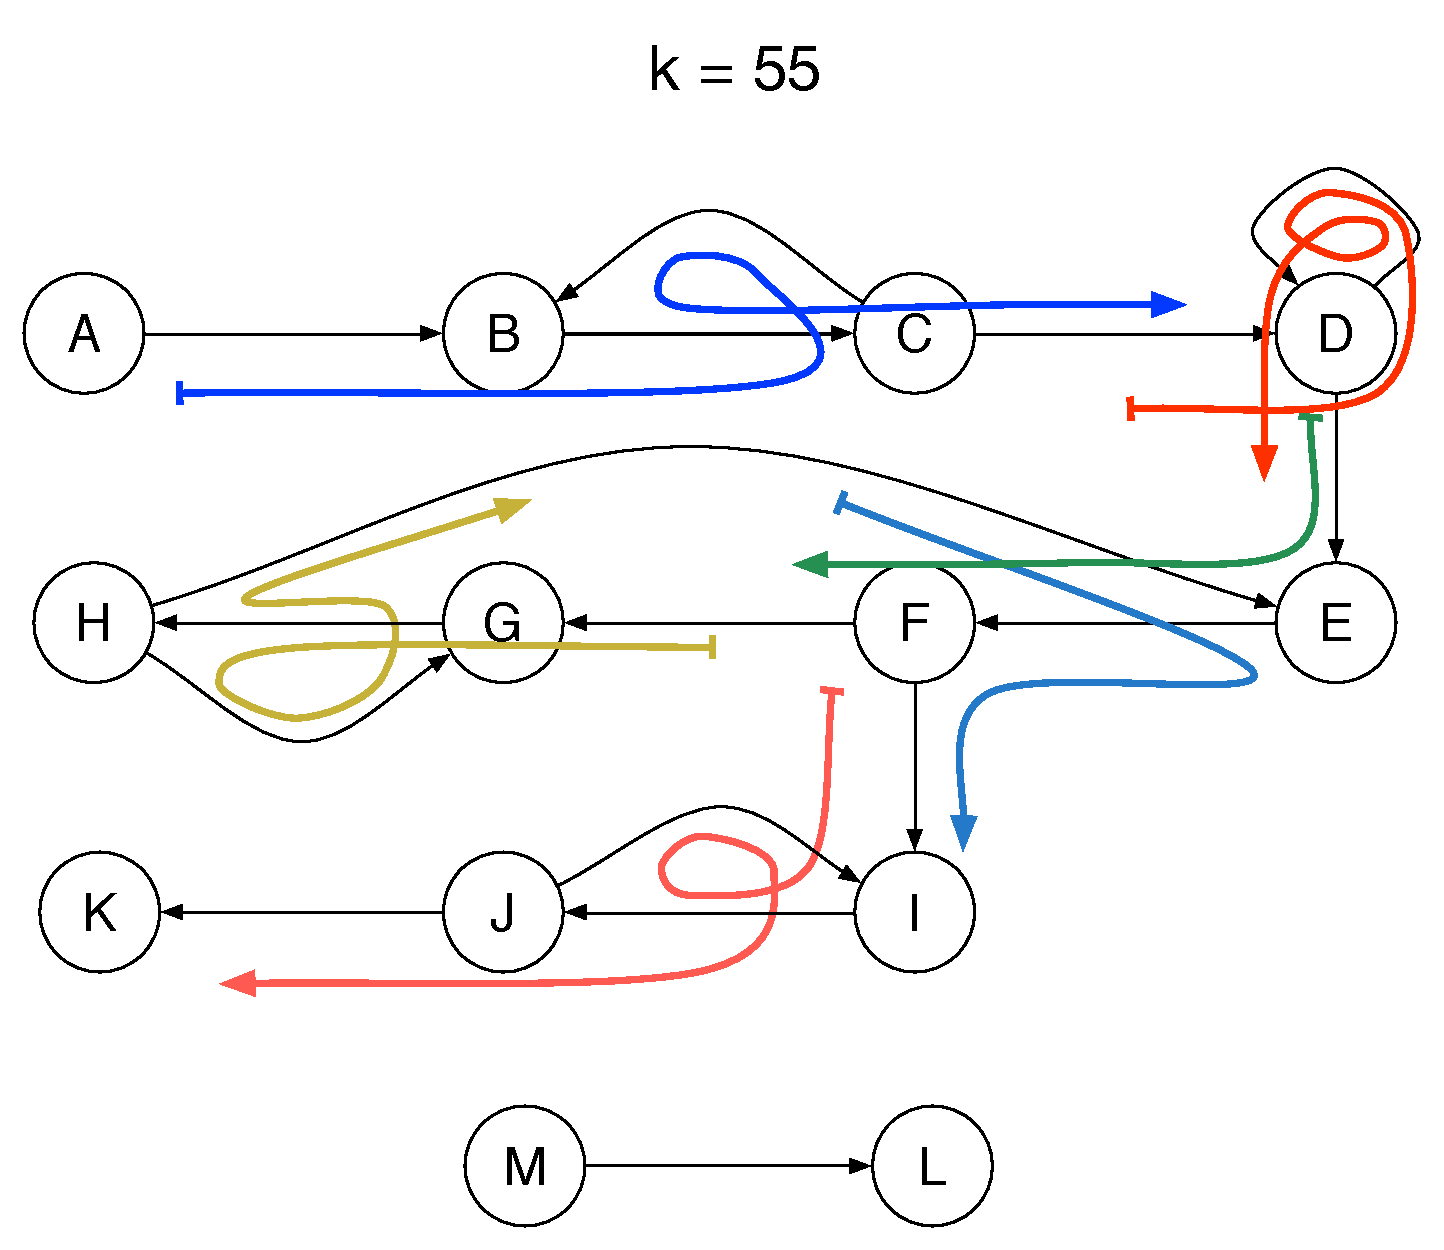
\includegraphics[scale=0.6]{k55.pdf}
  \end{center}
  \caption{Simüle edilmiş BYK verilerinden oluşturulan hiperçizge.}
  \label{fig:bac-hypergraph}
\end{figure}




\clearpage

\noindent
{\bf \large 4.4. Ekzom Dizilemede GC ve Yakalama Verimi Hatalarının Düzeltilmesi}
\addcontentsline{toc}{subsection}{4.4. Ekzom Dizilemede GC ve Yakalama Verimi Hatalarının Düzeltilmesi}

\paragraph{Korelasyon değerleri} 

Şekil \ref{fig:captureeff}'da 1000 Genom Projesi'ne~\cite{1000GP2012} ait rastgele seçilmiş 7 örneğe ait her bir ekzon bölgesindeki prob etkinliği ve dizi derinliği grafikte gösterilmektedir. Ayrıca korelasyon katsayıları da Tablo~\ref{tab:correlation}'da verilmiştir. Bu verilerdeki gürültüleri azaltabilmek için 1000 genom projesi kapsamındaki örneklerin her birinde ortak olarak bulunan delesyon, insersiyon ve düşük kapsama bölgeleri çıkarıldı. 

\begin{figure}[htb]
\begin{center}
  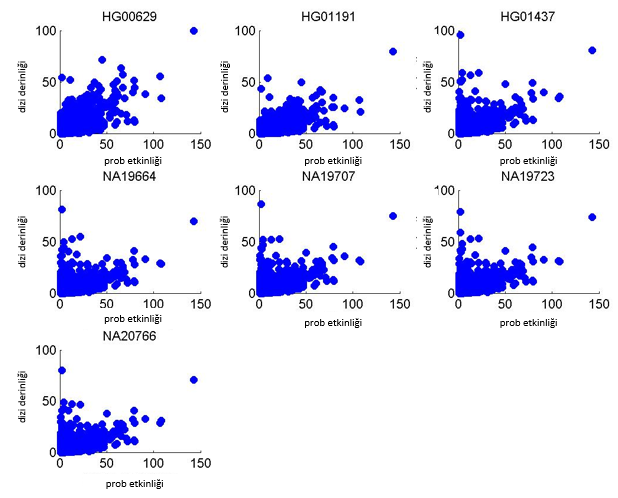
\includegraphics[scale=0.65]{captureeff.png}
\end{center}
\caption{Her bir ekzon bölgesine ait dizi derinliği ve prob yakalama etkinliği.}
\label{fig:captureeff}
\end{figure}

\begin{table}[htb]
\caption{1000 Genom Projesi'nden 7 örneğin dizileme derinliği (RD), prob sayısı (PR) ve GC içeriği (GC) ile korelasyonları.}
\label{tab:correlation}
\begin{center}
\begin{tabular}{|l|c|c|}
\hline 
{\bf Örnek } & {\bf RD-PR} & {\bf RD-PR-GC}\\
\hline 
HG00629 & 0.6478 & 0.7118\\
HG01191 & 0.6375 & 0.7095\\
HG01437 & 0.6483 & 0.6708\\
NA19664 & 0.6383 & 0.6640\\
NA19707 & 0.6484 & 0.6733\\
NA19723 & 0.6508 & 0.6751\\
NA20766 & 0.6509 & 0.6768\\
\hline
\end{tabular}
\end{center}
\vspace*{0.5cm}
 Görüldüğü üzere PR ve GC değerleri birlikte alınıp çoklu korelasyon hesaplandığında daha yüksek korelasyon katsayısı elde edilmektedir.
\end{table}

 Şekil \ref{fig:captureeff}'de de görüldüğü gibi gürültünün azaltılmasına rağmen prob kapsama etkinliği ve dizi derinliği arasında yeteri kadar güçlü bir ilişki bulunamamıştır. Daha sonra genom üzerinde bulunan her bir bazın kendisine yakın olan dizilimlerden etkilendiği düşüncesinden yola 
çıkarak, her bir genin içindeki ekzonları bir bütün olarak düşündük (Şekil \ref{fig:captureeffgene}).

\begin{figure}[htb]
\begin{center}
  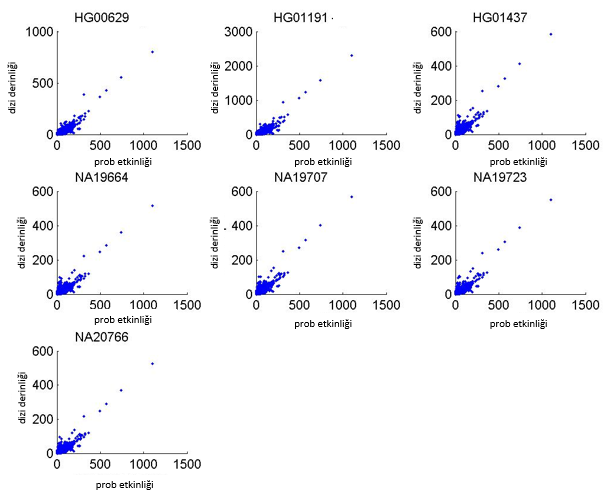
\includegraphics[scale=0.65]{captureeff-gene.png}
\end{center}
\caption{Her bir gen bölgesine ait dizi derinliği ve prob yakalama etkinliği.}
\label{fig:captureeffgene}
\end{figure}

  Sonuç olarak ekzonları ayrı ayrı ele almak yerine her bir gen bölgesinde bulunan ekzonları bir bütün olarak gördüğümüzde prob yakalama etkinliği ve dizi derinliği arasındaki ilişkinin güçlendiğini gözlemledik. Daha sonra datada bulunan prob etkinliği sapmasını düzeltebilmek için LOESS metodunu kullandık ve dizileme derinliğindeki hataları önemli ölçüde giderdik (Şekil~\ref{fig:captureeffloess}). Bu yöntem serpme diyagramında yerel olarak pürüzleri düzeltmede kullanılmaktadır.


\begin{figure}[htb]
\begin{center}
  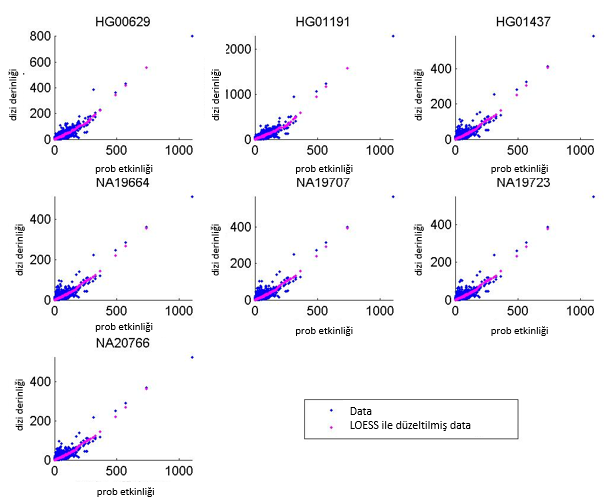
\includegraphics[scale=0.65]{captureeff-loess.png}
\end{center}
\caption{LOESS yöntemi kullanılarak düzeltilen veriler.}
\label{fig:captureeffloess}
\end{figure}

LOESS metoduyla düzeltilen data kullanılarak, ekzom birleştirme yöntemini daha doğru bir şekilde yapmak mümkün olacaktır.

\clearpage

\begin{center}
{\bf \Large 5. SONUÇ}
\end{center}
\addcontentsline{toc}{section}{5. SONUÇ}

\noindent
Yeni nesil dizileme (YND) teknolojileri sayesinde bütün biyolojik bilimlerdeki çalışma yöntemleri radikal bir şekilde değişmiştir. Ayrıca YND tıpta da kullanılmaya başlanmış ve kişileştirilmiş tıp alanının doğmasına yol açmıştır. Bu teknolojiler üretilen verilerin özellikleri ve maliyetleri konusunda da çok çeşitlilik gösterir, ve hemen hemen her 3-4 ayda bir yeni bir teknoloji piyasaya çıkmakta, ya da var olan bir dizileme platformunun yeni versiyonları piyasaya sürülmektedir. 2007 yılında Roche/454 ile başlayan YND serüveni, Illumina, SOLiD, Complete Genomics, Ion Torrent gibi kısa dizileme teknolojileri ile devam etmiş, son 1-2 yılda da PacBio, Oxford Nanopore (ONP) gibi uzun, ancak çok hata paylı dizileme teknolojileri safhasına geçilmiştir. Çok daha yakın zamanda 10X Genomics, Dövetail Genomics, ve CPT-Seq~\cite{Adey2014,Amini2014} gibi kısa Illumina okumalarını oluştururken uzun müleküllerdeki devamlılığı da takip edebilen yeni kütüphane hazırlama teknolojileri de ortaya çıkmıştır. YND platformlarındaki bu çeşitlilik de dizileme ve analiz yöntemlerinin özellikler klinik ortamda kullanımının standartlara oturtulmasını amaçlayan Genome in a Bottle Projesi'nin~\cite{Zook2014} başlamasına sebep olmuştur.

Yukarıda da belirttiğimiz üzere, her YND platformunun ürettiği veri dizi uzunluğu, hata profili ve maliyet gibi konularda birbirinden farklıdır. Ancak, bir teknoloji için dezavantaj olan bir özellik bir başka teknolojide avamtaja dönüşebilmektedir, ve bu artı-eksi farklılıkları birbirine paralel ilerler (çiftlilik prensibine [principle of dualıty] benzer şekilde). Örneğin, Illumina okumalarının kısa olmasına karşın PacBio ve ONP verileri uzundur, ancak buna karşılık Illumina'da hata payı binde 1'den az iken, PacBio'da \%15, ONP'de \%20 civarındadır. Bu nedenle, özellikle büyük genomların birleştirilmesi projelerinde aynı anda birden fazla YND platformunun verilerinden faydalanmak avantajlı olacaktır. Böylece genomdaki tekrarlar uzun PacBio ve ONP okumaları ile daha rahat çözümlenirken, hemen hemen hatasız Illumina verileri ile baz çifti düzeyindeki hatalar en aza indirgenecektir.

112E135 projesinde aynı anda birden fazla YND verişi kullanılarak genom birleştirmelerdeki hataların en aza indirgenmesi üzerine çalıştık:

\begin{itemize}
\item Roche/454, Ion Torrent ve Illumina verilerini birlikte kullanarak geliştirdiğimiz BYK birleştirmelerindeki hata düzeltimi algorıtması ÇİBB konferansında sunulmuştur~\cite{Kavak2015a} ve dergide çıkacak versiyonu üzerinde çalışmalarımız sürmektedir.
\item Illumina verilerini kullanarak PacBio okumalarındaki hataların düzeltilmesi için hızlı hizalama ve filtreleme algoritmamız küçük veri kümelerinde iyi çalışmaktadır. Ancak bu algoritmanın genom ölçeğinde de çalışabilmesi için implementasyonunda düzeltmeler gerekmektedir. Bu konuda Bilkent Üniversitesi'nde yüksek lisansına yeni başlayan Can Fırtına çalışacaktır.
\item Illumina ve PacBio okumalarını hipercizge üzerinde entegre ederek genom birleştirmesi algoritmamızın prototipi BYK büyüklüğünde ve simülasyon ile elde edilmiş verilerle çalışmaktadır. Bu prototip algoritmamız Bertinoro Computational Biology Meeting'de sunulmuştur~\cite{Ashyralyyev2015}. Gerçek veriler üzerinde denemelerimiz sürmektedir, bu algoritmamızın son versiyonunu da RECOMB konferansında sunmayı ve Bioinformatics dergisinde yayınlamayı planlamaktayız.
\end{itemize}

\noindent
{\bf \Large 5.1. Öneriler}
\addcontentsline{toc}{section}{5.1. Öneriler}
YND platformları arasındaki farklılıklardan dolayı, birden fazla YND teknolojisi ile elde edilmiş verilerin kullanılmasının genom birleştirmelerinin kalitesine pozitif bir etki sağladığı görülmüştür. Illumina'nın ucuz, PacBio ve ONP'nin ise görece pahalı teknolojiler olması nedeniyle, az maliyetli olduğu halde yüksek doğruluklu genom birleştirmelerini elde edebilmek için, çok yüksek derinlikte Illumina ($>$100X), ve düşük derinlikte PacBio/ONP ($>$5X) okumalarının entegre bir şekilde kullanılması uygun olacaktır. Bu verilere bütçe yeterliyse orta derinlikte Ion Torrent verilerinin ($\sim$8-9X) eklenmesinin de katkısı olabilir.

Ayrıca, gene yukarıda belirtildiği üzere, yeni dizileme teknolojileri (ONP gibi), kütüphane hazırlama protokolleri (10X Genomics, Dovetail Genomics, CPT-Seq, havuzlanmış klon dizileme), ve nanoteknoloji temelli DNA görüntüleme teknolojileri (BioNano) halen geliştirilmeye devam etmektedir. Bu yeni veri tıplerinin de etkin bir şekilde kullanımı için yeni algorıtma dizaynlarına ihtiyaç vardır. Genome in a Bottle Projesi, amaçları nedeniyle, hemen hemen her teknolojiden elde edilen verileri üretmektedir. Bu projeye katılım ile hem alandaki yeniliklerden anında haber olmak, hem de en yeni veriye anında erişim mümkün olmaktadır.

{\small 
\bibliographystyle{plain}
\bibliography{calkan}

}




\label{endsectionb1}
\end{document}
